% Options for packages loaded elsewhere
% Options for packages loaded elsewhere
\PassOptionsToPackage{unicode}{hyperref}
\PassOptionsToPackage{hyphens}{url}
\PassOptionsToPackage{dvipsnames,svgnames,x11names}{xcolor}
%
\documentclass[
  letterpaper,
  DIV=11,
  numbers=noendperiod]{scrreprt}
\usepackage{xcolor}
\usepackage{amsmath,amssymb}
\setcounter{secnumdepth}{5}
\usepackage{iftex}
\ifPDFTeX
  \usepackage[T1]{fontenc}
  \usepackage[utf8]{inputenc}
  \usepackage{textcomp} % provide euro and other symbols
\else % if luatex or xetex
  \usepackage{unicode-math} % this also loads fontspec
  \defaultfontfeatures{Scale=MatchLowercase}
  \defaultfontfeatures[\rmfamily]{Ligatures=TeX,Scale=1}
\fi
\usepackage{lmodern}
\ifPDFTeX\else
  % xetex/luatex font selection
\fi
% Use upquote if available, for straight quotes in verbatim environments
\IfFileExists{upquote.sty}{\usepackage{upquote}}{}
\IfFileExists{microtype.sty}{% use microtype if available
  \usepackage[]{microtype}
  \UseMicrotypeSet[protrusion]{basicmath} % disable protrusion for tt fonts
}{}
\makeatletter
\@ifundefined{KOMAClassName}{% if non-KOMA class
  \IfFileExists{parskip.sty}{%
    \usepackage{parskip}
  }{% else
    \setlength{\parindent}{0pt}
    \setlength{\parskip}{6pt plus 2pt minus 1pt}}
}{% if KOMA class
  \KOMAoptions{parskip=half}}
\makeatother
% Make \paragraph and \subparagraph free-standing
\makeatletter
\ifx\paragraph\undefined\else
  \let\oldparagraph\paragraph
  \renewcommand{\paragraph}{
    \@ifstar
      \xxxParagraphStar
      \xxxParagraphNoStar
  }
  \newcommand{\xxxParagraphStar}[1]{\oldparagraph*{#1}\mbox{}}
  \newcommand{\xxxParagraphNoStar}[1]{\oldparagraph{#1}\mbox{}}
\fi
\ifx\subparagraph\undefined\else
  \let\oldsubparagraph\subparagraph
  \renewcommand{\subparagraph}{
    \@ifstar
      \xxxSubParagraphStar
      \xxxSubParagraphNoStar
  }
  \newcommand{\xxxSubParagraphStar}[1]{\oldsubparagraph*{#1}\mbox{}}
  \newcommand{\xxxSubParagraphNoStar}[1]{\oldsubparagraph{#1}\mbox{}}
\fi
\makeatother


\usepackage{longtable,booktabs,array}
\newcounter{none} % for unnumbered tables
\usepackage{calc} % for calculating minipage widths
% Correct order of tables after \paragraph or \subparagraph
\usepackage{etoolbox}
\makeatletter
\patchcmd\longtable{\par}{\if@noskipsec\mbox{}\fi\par}{}{}
\makeatother
% Allow footnotes in longtable head/foot
\IfFileExists{footnotehyper.sty}{\usepackage{footnotehyper}}{\usepackage{footnote}}
\makesavenoteenv{longtable}
\usepackage{graphicx}
\makeatletter
\newsavebox\pandoc@box
\newcommand*\pandocbounded[1]{% scales image to fit in text height/width
  \sbox\pandoc@box{#1}%
  \Gscale@div\@tempa{\textheight}{\dimexpr\ht\pandoc@box+\dp\pandoc@box\relax}%
  \Gscale@div\@tempb{\linewidth}{\wd\pandoc@box}%
  \ifdim\@tempb\p@<\@tempa\p@\let\@tempa\@tempb\fi% select the smaller of both
  \ifdim\@tempa\p@<\p@\scalebox{\@tempa}{\usebox\pandoc@box}%
  \else\usebox{\pandoc@box}%
  \fi%
}
% Set default figure placement to htbp
\def\fps@figure{htbp}
\makeatother





\setlength{\emergencystretch}{3em} % prevent overfull lines

\providecommand{\tightlist}{%
  \setlength{\itemsep}{0pt}\setlength{\parskip}{0pt}}



 


\KOMAoption{captions}{tableheading}
\makeatletter
\@ifpackageloaded{tcolorbox}{}{\usepackage[skins,breakable]{tcolorbox}}
\@ifpackageloaded{fontawesome5}{}{\usepackage{fontawesome5}}
\definecolor{quarto-callout-color}{HTML}{909090}
\definecolor{quarto-callout-note-color}{HTML}{0758E5}
\definecolor{quarto-callout-important-color}{HTML}{CC1914}
\definecolor{quarto-callout-warning-color}{HTML}{EB9113}
\definecolor{quarto-callout-tip-color}{HTML}{00A047}
\definecolor{quarto-callout-caution-color}{HTML}{FC5300}
\definecolor{quarto-callout-color-frame}{HTML}{acacac}
\definecolor{quarto-callout-note-color-frame}{HTML}{4582ec}
\definecolor{quarto-callout-important-color-frame}{HTML}{d9534f}
\definecolor{quarto-callout-warning-color-frame}{HTML}{f0ad4e}
\definecolor{quarto-callout-tip-color-frame}{HTML}{02b875}
\definecolor{quarto-callout-caution-color-frame}{HTML}{fd7e14}
\makeatother
\makeatletter
\@ifpackageloaded{bookmark}{}{\usepackage{bookmark}}
\makeatother
\makeatletter
\@ifpackageloaded{caption}{}{\usepackage{caption}}
\AtBeginDocument{%
\ifdefined\contentsname
  \renewcommand*\contentsname{Table of contents}
\else
  \newcommand\contentsname{Table of contents}
\fi
\ifdefined\listfigurename
  \renewcommand*\listfigurename{List of Figures}
\else
  \newcommand\listfigurename{List of Figures}
\fi
\ifdefined\listtablename
  \renewcommand*\listtablename{List of Tables}
\else
  \newcommand\listtablename{List of Tables}
\fi
\ifdefined\figurename
  \renewcommand*\figurename{Figure}
\else
  \newcommand\figurename{Figure}
\fi
\ifdefined\tablename
  \renewcommand*\tablename{Table}
\else
  \newcommand\tablename{Table}
\fi
}
\@ifpackageloaded{float}{}{\usepackage{float}}
\floatstyle{ruled}
\@ifundefined{c@chapter}{\newfloat{codelisting}{h}{lop}}{\newfloat{codelisting}{h}{lop}[chapter]}
\floatname{codelisting}{Listing}
\newcommand*\listoflistings{\listof{codelisting}{List of Listings}}
\makeatother
\makeatletter
\makeatother
\makeatletter
\@ifpackageloaded{caption}{}{\usepackage{caption}}
\@ifpackageloaded{subcaption}{}{\usepackage{subcaption}}
\makeatother
\usepackage{bookmark}
\IfFileExists{xurl.sty}{\usepackage{xurl}}{} % add URL line breaks if available
\urlstyle{same}
\hypersetup{
  pdftitle={The Learn-It-All Educator},
  pdfauthor={Dr.~Szymon Machajewski},
  colorlinks=true,
  linkcolor={blue},
  filecolor={Maroon},
  citecolor={Blue},
  urlcolor={Blue},
  pdfcreator={LaTeX via pandoc}}


\title{The Learn-It-All Educator}
\usepackage{etoolbox}
\makeatletter
\providecommand{\subtitle}[1]{% add subtitle to \maketitle
  \apptocmd{\@title}{\par {\large #1 \par}}{}{}
}
\makeatother
\subtitle{A Guidebook for Training Brains, Not Replacing Them with AI}
\author{Dr.~Szymon Machajewski}
\date{2026-03-15}
\begin{document}
\maketitle

\renewcommand*\contentsname{Table of contents}
{
\setcounter{tocdepth}{2}
\tableofcontents
}

\bookmarksetup{startatroot}

\chapter{The Learn-It-All Educator}\label{the-learn-it-all-educator}

\frontmatter
\begin{titlepage}
\centering
\vspace*{2cm}
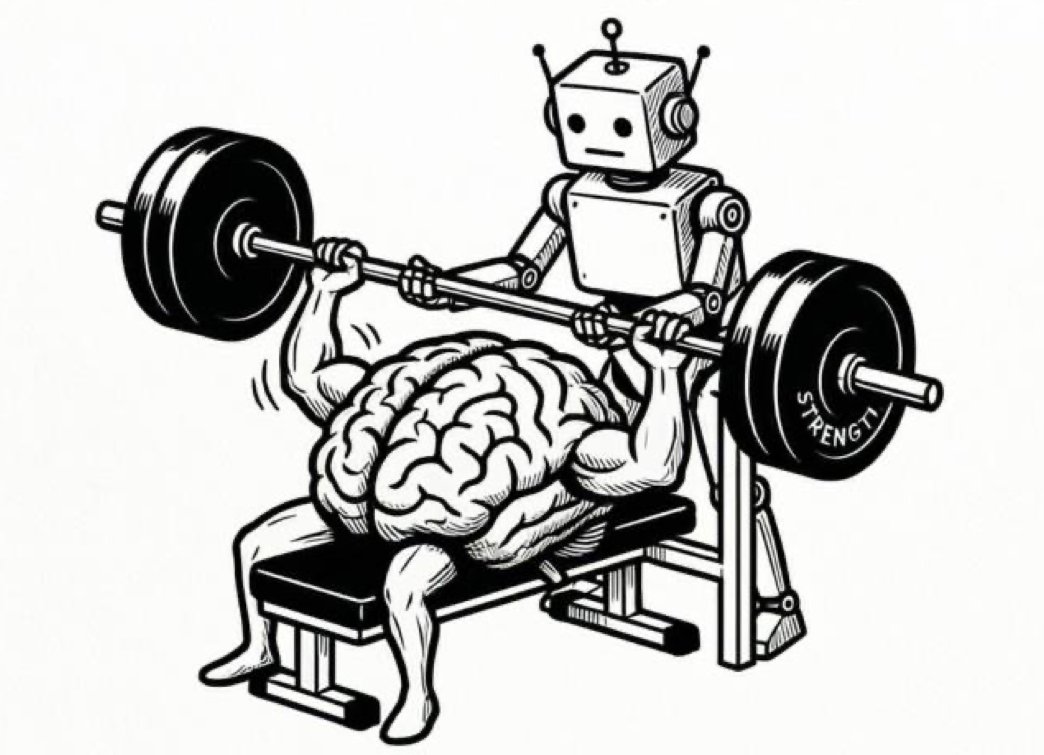
\includegraphics[width=0.55\textwidth]{cover.png}
\vspace{1.5cm}

{\LARGE\bfseries The Learn-It-All Educator}

\vspace{0.3cm}
{\large A Guidebook for Training Brains, Not Replacing Them with AI}

\vspace{0.5cm}
{\itshape Rethinking AI in Higher Education}

\vspace{1.5cm}
Dr. Szymon Machajewski

\vspace{0.5cm}
{\small DOI: \href{https://doi.org/10.5281/zenodo.19041123}{10.5281/zenodo.19041123}}
\end{titlepage}

\newpage
\thispagestyle{empty}
\vspace*{\fill}

{\small
Copyright © 2026 Szymon Machajewski

This work is licensed under a Creative Commons Attribution 4.0 International License (CC BY 4.0). You are free to share and adapt this work with proper attribution.

\vspace{0.5cm}
\textbf{Recommended Citation:}

Machajewski, S. (2026). \textit{The Learn-It-All Educator: A Guidebook for Training Brains, Not Replacing Them with AI}. Zenodo. \href{https://doi.org/10.5281/zenodo.19041123}{https://doi.org/10.5281/zenodo.19041123}

\vspace{0.5cm}
Version 1.2, March 2026

In collaboration with Lansing Community College, Center for Teaching Excellence

Companion site: \href{https://dataii.com/ai/guidebook}{dataii.com/ai/guidebook}
}

\vspace*{\fill}
\newpage

\bookmarksetup{startatroot}

\chapter{```}\label{section}

\mainmatter
number-sections: false
title: "Introduction: As a Human Thinketh, Our Learning Mindset"
subtitle: "Training Brains, Not Replacing Them"
lang: en
---

```{=latex}
\mainmatter

\subsection{The Trap}\label{the-trap}

There is a fear spreading through higher education, and it is not
unfounded.

The fear is this: artificial intelligence is destroying our ability to
think. Students are outsourcing their essays to ChatGPT. Faculty are
watching assignments return that clearly were not written by human
hands. The fundamental transaction of education - the exchange of effort
for learning - seems to be collapsing. We are educating students to
become their own replacements. Interchangeable cogs with credentials.

The research validates the concern. MIT scientists scanned the brains of
people writing essays and found something troubling. Those who relied
heavily on AI showed significantly weaker neural connectivity than those
who wrote independently. After four months, the AI-dependent group
performed measurably worse on cognitive tests. They were becoming less
capable of complex thought - not because they lacked intelligence, but
because they had stopped exercising it (Kosmyna et al., 2025,
arXiv:2506.08872).

The technical term is \emph{cognitive atrophy}. The brain, like any
muscle, loses strength when it stops working. And AI offers the most
seductive shortcut in the history of education: the ability to produce
sophisticated-looking work without the struggle that produces actual
learning.

The most vulnerable population? Young adults aged 20 to 30 - precisely
the students in our classrooms. Entry-level cognitive work, the kind
that builds professional capability, is exactly the work AI can now
perform. If students outsource that work throughout their education,
they graduate with credentials but without the underlying competence
those credentials are supposed to represent. They have the diploma. They
lack the mind.

This is the trap. And if we respond to it poorly - by either banning AI
entirely or surrendering to it completely - we will fail our students
and ourselves.

{[}p.~5{]}

\subsection{The Shift}\label{the-shift}

But there is another way to understand what is happening. The trap
becomes visible only when we think of AI as a tool for getting answers.
Reframe it as a tool for training the brain, and everything changes.

Consider the difference between two students preparing for an exam. The
first pastes the study material into ChatGPT, asks it to summarize the
key points, reads the summary, and calls it preparation. The second
pastes the same material into the AI and says: ``Quiz me on this
concept. Start at a basic level, then increase the difficulty until I
fail. Challenge every answer I give. Point out the weaknesses in my
reasoning.''

The first student used AI to \emph{remove} friction from learning. The
second used AI to \emph{add} friction - to create a more challenging,
more demanding learning experience than they could have created alone.
Same tool. Opposite outcomes.

This is the shift at the heart of this guidebook. AI is not inherently
good or bad for learning. It is an \emph{amplifier}. It amplifies
whatever intention you bring to it. If your intention is to avoid
cognitive effort, AI will help you avoid it magnificently. If your
intention is to challenge yourself more rigorously than ever before, AI
will help you do that too.

The question is not whether to use AI in education. That question has
been answered by reality - AI is here, students are using it, and
prohibition is both unenforceable and counterproductive. The question is
\emph{how} to use it: as an elevator that skips the climb, or as a gym
that builds strength.

\subsection{The Goal}\label{the-goal}

Higher education has always rewarded the ``know-it-all.'' Faculty are
hired for expertise, promoted for publications, respected for command of
their field. The entire professional identity is built on knowing things
that others do not.

But knowledge is changing faster than at any point in human history.
What was current five years ago may be obsolete today. The expert who
cannot become a beginner again is an expert with an expiration date. The
know-it-all who stops learning becomes the know-it-all who knows less
and less about more and more.

Consider the surgical profession - the epitome of the know-it-all
expert. Surgeons master anatomy, pharmacology, and surgical techniques
through a decade of grueling training. Yet despite this expertise,
surgical complications and deaths remained stubbornly high, even as
medicine grew more complex. Harvard surgeon Atul Gawande diagnosed the
problem: it was not lack of knowledge - it was failure to \emph{apply}
knowledge reliably. Even the most brilliant surgeon cannot hold every
detail of complex procedures in working memory.

Gawande's solution was deceptively simple: a 19-item checklist used
before, during, and after surgery. This ``unintelligent'' tool forced
surgeons to pause, communicate with teams, confirm critical steps, and
double-check for errors. The results were staggering. In WHO pilot
hospitals across eight countries, major complications fell 36\% and
deaths dropped 47\% (Haynes et al., 2009).

{[}p.~6{]} The checklist did not replace expertise - it \emph{protected}
it, turning know-it-all surgeons into learn-it-all teams willing to
embrace systematic humility.

The lesson applies directly to higher education. The goal of this
guidebook is to help educators make the same shift - from know-it-all to
\emph{learn-it-all}. Not because expertise is unimportant, but because
expertise without systematic humility becomes obsolescence. The true
master is a student for life.

\textbf{\emph{``The learn-it-all does better than the know-it-all.''}}\\
\emph{Satya Nadella, CEO of Microsoft (Bloomberg Businessweek, 2016)}

\subsection{What This Guidebook
Offers}\label{what-this-guidebook-offers}

This guidebook provides four frameworks for thriving as an educator in
the age of AI. Each chapter addresses a different dimension of the
challenge:

{\def\LTcaptype{none} % do not increment counter
\begin{longtable}[]{@{}
  >{\raggedright\arraybackslash}p{(\linewidth - 0\tabcolsep) * \real{1.0000}}@{}}
\toprule\noalign{}
\endhead
\bottomrule\noalign{}
\endlastfoot
\textbf{Chapter 1: Cognitive Triage} Not all tasks deserve equal effort.
This chapter introduces the FLUFF/SPARK framework for distinguishing
work worth delegating (Formatting, Layouts, Under-the-hood, Filing,
Filtering) from ideas worth thinking (Specific, Persuasive, Authentic,
Rigorous, Keen-insight). Delegate the FLUFF to AI; reserve your
cognitive energy for the SPARK. \\
\textbf{Chapter 2: The Intelligent Gearbox} AI is a probability engine,
not a calculator - it predicts likely word sequences rather than
retrieving verified facts. Understanding this changes how you should
interact with it. This chapter presents a progression of prompting
techniques - from first gear through overdrive - and reveals how the
same principles that improve AI prompts also improve teaching. \\
\textbf{Chapter 3: The Cognitive Gym} When it comes to student learning,
the goal is not to remove friction but to add it strategically. This
chapter introduces Progressive Overload (using AI as a coach that
increases challenge), the Verification Protocol (a five-step AI Audit
that shifts assessment from generation to verification), and the VINE
Framework (developing the taste that distinguishes average from
excellent). Together, these frameworks make ``zombie submissions'' far
more difficult. \\
\textbf{Chapter 4: The Intelligent Simpleton} The greatest obstacle to
learning is not ignorance but ego - the need to appear as a know-it-all.
Neuroplasticity happens at the edge of ability, which means feeling lost
or like a beginner again is the condition for growth, not an obstacle to
it. This chapter explores how to use AI as a judgment-free zone for
asking basic questions, how to overcome authenticity and institutional
barriers, and why the courage to play the simpleton today is the path to
remaining the scholar and a well-prepared, learn-it-all educator
tomorrow. \\
\end{longtable}
}

\subsection{How to Use This Guidebook}\label{how-to-use-this-guidebook}

This guidebook is designed for practical application, not passive
reading. Each chapter includes:

\begin{itemize}
\tightlist
\item
  Conceptual frameworks that reframe how you think about AI in education
\item
  {[}p.~7{]} Concrete practices you can implement immediately
\item
  Sample prompts and assignment structures ready for adaptation
\item
  Key takeaways summarizing the essential points
\end{itemize}

You do not need to read the chapters in order, though they build on each
other. If your immediate concern is reclaiming time from administrative
work, start with Chapter 1. If you are struggling with assignment design
in an AI world, go directly to Chapter 3. If you simply feel overwhelmed
by the pace of technological change, Chapter 4 may be the place to
begin.

The frameworks in this guidebook are not theoretical. They emerge from
the lived experience of educators navigating the AI transition, from
research on learning and cognition, and from hard-won lessons about what
works and what does not. They will evolve as the technology evolves.
Consider this a living document - a starting point for your own
experimentation and adaptation.

\subsection{A Note on the Stakes}\label{a-note-on-the-stakes}

We are living through a transformation comparable to the introduction of
the printing press, the development of electricity, or the invention of
the internet. Throughout human history, we have faced technological
disruptions that seemed overwhelming at the time. We learned to control
fire, harness electricity, and split the atom. Each transition required
unlearning old assumptions and building new capabilities. Each produced
both remarkable benefits and serious risks.

AI is the latest chapter in this ongoing story. It will not be the last.
The same species that navigated those earlier transitions will navigate
this one. The question is whether we navigate it well or poorly -
whether we use these tools to expand human capability or to diminish it.

For educators, the stakes are high. We are not merely adapting to a new
technology. We are shaping how the next generation relates to that
technology. If we model thoughtful, critical, creative engagement with
AI, our students will learn that engagement. If we model avoidance or
uncritical dependence, they will learn that instead.

The good news is that the skills AI makes more valuable - critical
thinking, emotional intelligence, judgment under uncertainty, creative
intuition, and the ability to keep learning - are precisely the skills
that great educators have always cultivated. The age of AI does not make
good teaching obsolete. It makes good teaching essential.

The future of human intelligence is being written right now. You get to
help write it.

\subsection{What This Guidebook Does Not
Address}\label{what-this-guidebook-does-not-address}

This guidebook is written for educators who have decided to engage with
AI in their teaching. It is \emph{permissive} (here's how, if you
choose) rather than \emph{prescriptive} (you must do this). Thoughtful
critics have raised concerns that deserve acknowledgment, even if they
exceed what this guidebook can adequately address:

{[}p.~8{]} \textbf{On the evidence base.} The neuroscience research
cited (Kosmyna et al., 2025) is a preprint, not yet peer-reviewed.
Claims about cognitive benefits and harms of AI use remain emerging
science, not settled fact.

\textbf{On environmental and labor costs.} AI systems consume
significant energy, water, and computational resources. The ``free''
tools educators and students use are subsidized by venture capital, data
extraction, and - in some cases - underpaid content moderation labor.
This guidebook does not examine these costs.

\textbf{On data and privacy.} When educators and students interact with
AI platforms, that data may be used to train future models or inform
commercial products. The implications for academic privacy and
intellectual property remain unresolved.

\textbf{On the case for resistance.} This guidebook frames AI adoption
as a practical reality to navigate, not a choice to be weighed.
Legitimate pedagogical alternatives exist: handwritten work, synchronous
assessment, AI-free course designs, and curricula that deliberately
preserve struggle without technological scaffolding. Educators who
choose these approaches are not Luddites - they may be protecting values
(deep reading, unassisted thinking, embodied learning) that this
guidebook underweights.

\textbf{On academic freedom.} Nothing in this guidebook should be read
as pressure to adopt AI. Educators have the right to design AI-minimal
or AI-free courses based on their disciplinary values and pedagogical
philosophy. A mathematics instructor who believes unassisted struggle is
essential to learning, or an English professor committed to close
reading without AI summaries, is making a defensible choice this
guidebook does not challenge.

These limitations are not weaknesses to be fixed in a future edition -
they reflect genuine tensions that honest engagement with AI in
education requires acknowledging.

\textbf{\emph{The age of AI does not make good teaching obsolete.}}\\
\textbf{\emph{It makes good teaching essential.}}

\begin{center}\rule{0.5\linewidth}{0.5pt}\end{center}

\bookmarksetup{startatroot}

\chapter{Chapter 1: Cognitive Triage}\label{chapter-1-cognitive-triage}

Managing Educator Workload in the Age of AI

\hfill\break

\begin{tcolorbox}[enhanced jigsaw, arc=.35mm, bottomrule=.15mm, breakable, colback=white, colframe=quarto-callout-note-color-frame, left=2mm, leftrule=.75mm, opacityback=0, rightrule=.15mm, toprule=.15mm]

Machajewski, Szymon. (2026). \emph{The Learn-It-All Educator --- A
Guidebook for Training Brains, Not Replacing Them with AI}. Zenodo.
\url{https://doi.org/10.5281/zenodo.19041123} · CC BY 4.0

\end{tcolorbox}

{[}p.~9{]}

\textbf{\emph{Managing Educator Workload in the Age of AI}}

\textbf{Chapter Objective:} Reclaiming time from administrative tasks to
focus on high-impact pedagogy.

There is a quiet crisis unfolding in higher education, and it has
nothing to do with enrollment numbers or budget cuts. It is about how
educators spend their time. According to research from MIT, heavy
reliance on AI for cognitive tasks actually weakens neural connectivity
over time. In brain scans of people writing essays, those who used only
their own minds showed the strongest neural pathways, while heavy AI
users showed the weakest. After four months, the AI-dependent group
performed measurably worse on cognitive tests (Kosmyna et al., 2025,
arXiv:2506.08872).

This presents a paradox. If using AI carelessly atrophies the brain,
should we avoid it entirely? The answer is no. The solution lies in what
we might call \emph{cognitive triage} - the strategic deployment of AI
on tasks where perfection adds no value, precisely so we can pour our
full cognitive energy into the work that actually matters.

This chapter introduces two frameworks for doing exactly that. FLUFF
identifies the tasks worth delegating to AI - work that makes a course
look polished but does not build cognitive muscle. SPARK identifies the
ideas worth thinking - work where human judgment, creativity, and rigor
produce returns that AI cannot replicate. Together, they help you
distinguish between harvesting (where speed is good and automation makes
sense) and seeding (where investment, struggle, and growth create
lasting value).

\section{1.1 Harvesting vs.~Seeding: Two Types of Academic
Work}\label{harvesting-vs.-seeding-two-types-of-academic-work}

Not all tasks are created equal. Some have a ceiling on their value;
others have none. The first step toward cognitive triage and delegation
of thinking is learning to tell the difference.

Think of it as the difference between harvesting and seeding. When you
harvest, speed matters. The crop is ready; you need to collect it
efficiently before the weather turns. Automation helps you weather the
opportunity. But when you seed, speed is not the point. You are making
an investment with uncertain returns. You are nurturing something that
will grow over time. Rush the seeding, and you get nothing worth
harvesting later.

Academic work follows the same pattern. Some tasks are transactional -
get them done, move on, no additional value comes from obsessing over
them. These have \emph{capped payoffs}. Other tasks are growth-oriented
- the more you invest, the more you get back. These have \emph{uncapped
payoffs}. Pour your cognitive energy into the wrong category, and you
exhaust yourself polishing things that do not matter while neglecting
the work that could transform your students and your career.

\section{1.2 FLUFF: The Work Worth
Delegating}\label{fluff-the-work-worth-delegating}

FLUFF stands for Formatting, Layouts, Under-the-hood, Filing, and
Filtering. These are tasks with capped payoffs - work that makes a
course look ``pretty'' but does not build cognitive muscle.

{[}p.~10{]} Spending three hours perfecting these yields no additional
value over spending thirty minutes. They are harvesting tasks: get them
done efficiently and move on.

{\def\LTcaptype{none} % do not increment counter
\begin{longtable}[]{@{}
  >{\raggedright\arraybackslash}p{(\linewidth - 0\tabcolsep) * \real{1.0000}}@{}}
\toprule\noalign{}
\endhead
\bottomrule\noalign{}
\endlastfoot
\textbf{FLUFF: Formatting, Layouts, Under-the-hood, Filing,
Filtering} \\
\emph{Vibe:} Work that makes the course look polished but doesn't build
student muscle. \\
\end{longtable}
}

\subsection{F - Formatting}\label{f---formatting}

Polishing syllabi, fixing citation styles, ensuring consistent fonts
across documents - this work matters for professionalism but has
diminishing returns. A syllabus formatted to 80\% quality serves
students just as well as one formatted to 100\%. The extra 20\% is pure
FLUFF.

\emph{Examples:}

\begin{itemize}
\tightlist
\item
  Converting citations from APA to Chicago or MLA
\item
  Standardizing heading styles across course documents
\item
  Cleaning up inconsistent bullet formatting
\end{itemize}

\subsection{L - Layouts}\label{l---layouts}

Designing visual banners, perfecting PowerPoint slides, creating
aesthetically pleasing headers - this work can consume hours with
minimal pedagogical return. A serviceable layout communicates; a perfect
layout does not teach better.

\emph{Examples:}

\begin{itemize}
\tightlist
\item
  Creating course banners or visual headers for LMS pages
\item
  Perfecting slide deck aesthetics and transitions
\item
  Designing infographics for content that could be explained in text
\end{itemize}

\subsection{U - Under-the-hood}\label{u---under-the-hood}

Technical logistics that keep courses running but add no intellectual
value: fixing broken links, troubleshooting file formats, updating
embedded media. These are necessary but should not consume your limited
cognitive energy.

\emph{Examples:}

\begin{itemize}
\tightlist
\item
  Fixing broken hyperlinks in course materials
\item
  Converting files between formats (PDF to Word, etc.)
\item
  Troubleshooting LMS settings and permissions
\end{itemize}

\subsection{F - Filing}\label{f---filing}

Organizing unstructured data, categorizing qualitative feedback,
cleaning up messy gradebooks. This work is necessary for functioning
courses but is pure administration - no neural pathways are strengthened
by alphabetizing a folder.

\emph{Examples:}

\begin{itemize}
\tightlist
\item
  Categorizing open-ended survey responses into themes
\item
  {[}p.~11{]} Organizing student submissions into grading folders
\item
  Cleaning up spreadsheets of grades or attendance data
\end{itemize}

\subsection{F - Filtering}\label{f---filtering}

Sifting through search results, scanning long articles for specific
quotes, finding patterns in large datasets. AI excels at this - it can
fire off hundreds of secondary queries and surface relevant passages in
seconds. Use it.

\emph{Examples:}

\begin{itemize}
\tightlist
\item
  Scanning literature to identify relevant studies
\item
  Extracting key quotes from lengthy PDFs
\item
  Finding patterns in student feedback or course evaluations
\end{itemize}

Critical warning: AI filtering is powerful but dangerous. AI systems are
probability engines, not truth engines. They can hallucinate citations,
invent sources, and present fabricated information with complete
confidence. Use AI to narrow the field, but always verify what it
surfaces. Filtering is FLUFF; verification is SPARK.

\subsection{The FLUFF Mindset}\label{the-fluff-mindset}

The goal with FLUFF is not perfection - it is sufficiency. These are
transactional tasks with capped payoffs. Delegate them to AI, accept
``good enough,'' and reclaim the hours for work that matters.

Before any task, ask: Is this harvesting or seeding? If harvesting - if
speed is good and additional effort yields no additional value - let AI
handle it. Your cognitive energy is finite. Stop spending it on FLUFF.

\section{1.3 SPARK: Ideas Worth
Thinking}\label{spark-ideas-worth-thinking}

If FLUFF represents work worth delegating, SPARK represents ideas worth
thinking - the human edge where investment produces uncapped returns.
SPARK stands for Specific, Persuasive, Authentic, Rigorous, and
Keen-Insight. These are seeding activities: investments with risk but
potential for transformative growth.

\subsection{S - Specific}\label{s---specific}

\emph{Moving from Generalities to Insights}

AI operates at Unit 1 - the basics, the generalities, the consensus. It
produces what is most probable, most common, most expected. But
expertise lives at Unit 2 - the complex, the contested, the nuanced. The
specific insight that distinguishes your course from a generic textbook,
the precise example that illuminates a difficult concept for your
particular students, the unexpected connection between your discipline
and a current event - these require human judgment.

{[}p.~12{]} \textbf{SPARK in action:} When AI gives you a generic
framework, push it to specifics. ``This is useful but generic. What
would this look like for community college students returning to
education after a career change? What specific obstacles would they
face?'' The specificity is your contribution - and it is where the value
lives.

\subsection{P - Persuasive}\label{p---persuasive}

\emph{The Art of the Compelling Argument}

AI generates competent prose but rarely compelling argument. Persuasion
requires understanding your audience's specific fears, values, and
objections - and crafting an argument that meets them where they are. It
requires the kind of empathy that comes from genuine human interaction,
from knowing that this particular dean cares about retention numbers, or
that these particular students are skeptical of theoretical frameworks
because they are already working in the field.

\textbf{SPARK in action:} When you need to persuade a committee, a
department, or a student, do not outsource the argument to AI. Use AI to
check your logic, anticipate counterarguments, and improve your prose -
but the persuasive strategy must come from your understanding of the
audience.

\subsection{A - Authentic}\label{a---authentic}

\emph{Your Voice, Your Values, Your Mentorship}

Students can tell the difference between a professor who genuinely cares
and one who is going through the motions. Authenticity - the sense that
you are present, engaged, and personally invested in their growth -
cannot be replicated by AI. Mentorship, encouragement, the moment when
you recognize that a student is struggling and find the right words -
these are irreducibly human.

\textbf{SPARK in action:} When students submit writing, the question is
not ``did AI generate this?'' but ``is there a distinctive human voice
here?'' Mentor students in developing their authentic perspective - a
task that AI cannot perform and that produces uncapped returns in their
professional lives.

{[}p.~13{]}

\subsection{R - Rigorous}\label{r---rigorous}

\emph{Moving Beyond Transactional Tasks}

A transactional task is asking AI for an answer to save time. A growth
task is the rigorous audit of that answer. The first is harvesting; the
second is seeding. The first has capped payoff; the second builds the
neural connectivity that makes you (and your students) more capable over
time.

Rigor means checking AI's sources, questioning its assumptions,
demanding evidence for its claims. This is an investment of effort -
slower than accepting AI output at face value. But speed is for
harvesting. Rigor is the struggle that produces growth.

\textbf{SPARK in action:} When AI provides information, treat
verification as the real work. Does the citation exist? Does the source
actually say what AI claims? What would change if a key assumption were
wrong? This rigor is where learning happens - both for you and for
students you teach to do the same.

\subsection{K - Keen-Insight}\label{k---keen-insight}

\emph{The Uncapped Payoff of the Human Edge}

AI predicts the probable; humans sense the non-obvious. Keen-insight
represents the ultimate uncapped payoff - where a single risky or
original idea can transform a project, a course, a career.

Consider Michael Crow at Arizona State University. Over the past decade,
ASU has used online and hybrid programs to open access for
non-traditional students -- working adults, caregivers, and
career-changers who cannot relocate for a degree. Its fully online
student population grew from roughly 400 students in 2010 to more than
60,000 by 2020, with a publicly stated goal of 100,000 online
degree-seeking students by the mid-2020s. In high-enrollment gateway
courses like College Algebra, an adaptive learning redesign using ALEKS
increased the share of students earning a C or better from 57\% in 2012
to 85\% in 2019, an overall 17-percentage-point gain since 2015 (Every
Learner Everywhere, 2020). Crow's strategy turned ASU from a regional
institution into one of the world's largest laboratories for scaled
online learning.

\textbf{SPARK in action:} When AI gives you the probable answer, ask:
what might be true that the data does not show? What patterns are
emerging that have not yet reached statistical significance? What does
your experience suggest that contradicts the consensus? This is the
human edge - and it is where transformative value lives.

\section{Putting It Together: From FLUFF to
SPARK}\label{putting-it-together-from-fluff-to-spark}

The transition from FLUFF to SPARK is the transition from transactional
work to growth work, from capped payoffs to uncapped payoffs, from
harvesting to seeding. Both are necessary. The mistake is confusing
them.

Spend your cognitive energy on FLUFF, and you exhaust yourself on work
that machines can do - leaving nothing for the ideas worth thinking.
Delegate FLUFF to AI, and you reclaim hours for the SPARK work that
defines a meaningful career in education: the specific insights, the
persuasive {[}p.~14{]} arguments, the authentic mentoring, the rigorous
verification, the keen-insights that transform how students see the
world.

For community college educators especially, this distinction is
critical. Technical careers programs must constantly update curricula to
match rapidly changing industry standards. The time you save on FLUFF is
time you can spend ensuring your students learn the specific skills
employers actually need, developing authentic professional judgment, and
building the rigorous verification habits that separate competent
professionals from dangerous ones.

As we will see in the next chapter, how you interact with AI matters as
much as what you delegate to it. Basic prompting yields basic results.
The Intelligent Gearbox framework shows how to shift into higher
performance.

\subsection{Chapter 1 Key Takeaways}\label{chapter-1-key-takeaways}

\begin{enumerate}
\def\labelenumi{\arabic{enumi}.}
\tightlist
\item
  Distinguish between harvesting (transactional, capped payoff) and
  seeding (growth-oriented, uncapped payoff) tasks.
\item
  Delegate FLUFF to AI: Formatting, Layouts, Under-the-hood, Filing,
  Filtering.
\item
  Reserve your cognitive energy for SPARK: Specific, Persuasive,
  Authentic, Rigorous, Keen-Insight.
\item
  AI excels at Unit 1 (basics, generalities); humans own Unit 2
  (complex, nuanced, controversial).
\item
  Always verify AI filtering - use it to narrow the field, but rigor is
  where learning happens.
\item
  The goal is not to work less - it is to invest your effort where it
  produces uncapped returns.
\end{enumerate}

\begin{center}\rule{0.5\linewidth}{0.5pt}\end{center}

\begin{tcolorbox}[enhanced jigsaw, arc=.35mm, bottomrule=.15mm, bottomtitle=1mm, breakable, colback=white, colbacktitle=quarto-callout-note-color!10!white, colframe=quarto-callout-note-color-frame, coltitle=black, left=2mm, leftrule=.75mm, opacityback=0, opacitybacktitle=0.6, rightrule=.15mm, title=\textcolor{quarto-callout-note-color}{\faInfo}\hspace{0.5em}{Companion Worksheet}, titlerule=0mm, toprule=.15mm, toptitle=1mm]

The worksheet for this chapter is available at the companion website:
\href{https://dataii.com/ai/guidebook/\#:~:text=Cognitive\%20Triage\%20Worksheet}{Cognitive
Triage Worksheet}

\end{tcolorbox}

\bookmarksetup{startatroot}

\chapter{Chapter 2: The Intelligent
Gearbox}\label{chapter-2-the-intelligent-gearbox}

Advanced Prompting for Educators

\hfill\break

{[}p.~15{]}

\textbf{\emph{Advanced Prompting for Educators}}

\textbf{Chapter Objective:} Moving beyond basic questions to get elite
results from AI.

Chapter 1 established what to delegate to AI. This chapter addresses
something equally important: \emph{how} to communicate with it
effectively.

Most educators interact with AI the way they might search Google -
typing a question and hoping for a useful answer. This approach works
for simple queries, but it fails spectacularly for complex academic
tasks. The difference between mediocre AI output and genuinely useful
results often comes down to how you ask.

Think of prompting skill as a gearbox. In first gear, you ask basic
questions and get basic answers - you can move, but slowly. As you shift
into higher gears, your techniques become more sophisticated, and the
quality of AI output improves dramatically. This chapter will take you
from first gear to overdrive.

\section{2.1 AI Is a Probability
Engine}\label{ai-is-a-probability-engine}

Before learning to shift gears, you need to understand what you are
working with. Many people treat AI like a calculator - input a question,
receive a correct answer. This mental model is fundamentally wrong.

A calculator operates on certainty. When you enter 47 × 23, it returns
1,081 because mathematical operations have deterministic outcomes. AI
operates on \emph{probability}. When you ask a large language model a
question, it does not retrieve a stored answer. Instead, it predicts the
most likely sequence of words to follow your input, based on patterns
learned from training data. It is a probability engine - extraordinarily
sophisticated, but fundamentally engaged in statistical prediction
rather than factual retrieval.

This distinction has one critical implication: \emph{context shapes
output}. Because AI predicts based on patterns, the context you provide
heavily influences what it generates. Better context yields better
predictions. Vague prompts produce vague outputs. The quality of your
prompts directly determines the quality of your results.

Mastering the intelligent gearbox means learning to provide increasingly
sophisticated context - which is exactly what the four gears teach you
to do.

\section{2.2 Shifting Through the
Gears}\label{shifting-through-the-gears}

Most users never shift out of first gear. They type simple questions -
what researchers call zero-shot prompting - and accept whatever comes
back. This works for trivial tasks but produces unreliable results for
anything complex.

{[}p.~16{]} The prompting gearbox has four gears, each representing a
more sophisticated approach. As you shift up, you provide more context,
more structure, and more guidance - and the AI's outputs improve
correspondingly.

{\def\LTcaptype{none} % do not increment counter
\begin{longtable}[]{@{}
  >{\raggedright\arraybackslash}p{(\linewidth - 0\tabcolsep) * \real{1.0000}}@{}}
\toprule\noalign{}
\endhead
\bottomrule\noalign{}
\endlastfoot
\textbf{The Wrong Gear Problem} \\
Anyone who has driven a manual transmission knows the sound of being in
the wrong gear. First gear on the highway: the engine screams at 6,000
RPM while you crawl forward. Fourth gear from a dead stop: the engine
lugs, shudders, and stalls. AI prompting works the same way. \emph{First
gear for a highway task} - a basic prompt for a complex analysis -
produces shallow, generic output. \emph{Fourth gear from a dead stop} -
over-engineering a prompt for a simple question - wastes time and
confuses the AI. The grinding noise is the AI producing garbage because
prompt sophistication doesn't match task complexity. \\
\end{longtable}
}

\subsection{First Gear: One-Shot Prompting
(Contextualizing)}\label{first-gear-one-shot-prompting-contextualizing}

\textbf{Core Principle:} Never let the model guess blindly. Provide one
clear example so the AI understands what you want.

In neutral - what researchers call zero-shot prompting - users ask
questions with no examples. ``Write a feedback email to a student about
their failing grade.'' The AI has nothing to anchor on except its
general training, so it produces generic output that may not match your
voice, your institution's norms, or your pedagogical approach.

First gear solves this by providing a single example. Instead of asking
the AI to guess, you show it what success looks like.

\emph{Educator application:}

\emph{``Write a feedback email to a student about their failing grade.
Use this previous email I sent as a style guide for tone and structure:
{[}paste example email{]}.''}

The single example transforms the task. Now the AI is not inventing a
communication style - it is matching one you have already established.

\textbf{Key Insight:} \emph{The same principles that make AI produce
better outputs make students}\\
\emph{produce better learning. Scaffolding is not spoon-feeding - it is
good instructional design.}

\begin{center}\rule{0.5\linewidth}{0.5pt}\end{center}

\subsection{Second Gear: Few-Shot Prompting
(Grounding)}\label{second-gear-few-shot-prompting-grounding}

\textbf{Core Principle:} Provide three or more examples to ground the
model and reduce hallucinations.

Here is where the probability engine becomes dangerous. Because AI
predicts likely word sequences rather than retrieving verified facts, it
can generate plausible-sounding content that is completely fabricated.
It will invent citations to papers that do not exist. It will attribute
quotes to people who never said them. It will present fictional
statistics with the same confidence as real ones. AI researchers call
this \emph{hallucination} - and it happens most often when the model has
insufficient context to constrain its predictions.

{[}p.~17{]} Few-shot prompting is the antidote. By providing three or
more examples, you give the AI boundaries. Instead of predicting what
\emph{might} be appropriate based on its general training, it identifies
patterns across \emph{your specific instances}. The examples act as
guardrails, channeling the probability engine toward outputs that match
your actual standards rather than its statistical guesses.

This technique is particularly powerful for tasks involving style,
structure, or evaluation criteria - areas where a single example might
be idiosyncratic but multiple examples reveal consistent patterns.

\emph{Educator application:}

\emph{``Here are three of my previous successful essays that received
high marks. Based on these examples, write a structural outline for my
new essay on {[}topic{]}. Match my writing style and argumentative
approach.''}

With three examples, the AI can identify what makes your essays
successful - your paragraph structure, your use of evidence, your
argumentative moves - rather than defaulting to generic academic writing
conventions or inventing approaches that sound plausible but miss your
standards.

\textbf{Pro tip - the explanation technique:} Before asking the AI to
generate new content, ask it to explain the pattern back to you first.
This forces the model to articulate its understanding of what makes your
examples successful - and reveals whether it has actually grasped the
pattern or is about to hallucinate.

\textbf{Key insight:} Three examples are the minimum for reliable
pattern extraction. More examples increase consistency and reduce
hallucinations, especially for complex or nuanced tasks.

\textbf{Pro tip - grounding tools:} Tools like Google's NotebookLM take
grounding even further through a technique called Retrieval-Augmented
Generation (RAG). Upload your course materials, research articles, or
institutional documents, and the AI's responses are constrained
\emph{exclusively} to that content - with citations linking directly to
your sources. This dramatically reduces hallucinations for
discipline-specific work. NotebookLM also transforms your documents into
multiple output formats: Audio Overviews generate podcast-style
discussions between two AI hosts available in 80+ languages and
downloadable for offline listening. Video Overviews create visual
explainer presentations that pull images, diagrams, and key quotes from
your sources. Mind Maps provide interactive visual navigation of complex
topics. For educators, this means students can engage with course
readings through their preferred modality - reading, listening during a
commute, or watching a visual summary - all grounded in the exact
materials you assigned.

\subsection{Third Gear: Chain of Thought
Reasoning}\label{third-gear-chain-of-thought-reasoning}

\textbf{Core Principle:} Force the AI to show its work and think step by
step to reduce errors on complex problems.

{[}p.~18{]} For complex reasoning tasks - analysis, evaluation,
multi-step problem solving - the quality of AI output improves
dramatically when you explicitly require the model to externalize its
thinking process.

The magic phrase is simple: ``Think step by step'' or ``Show your
work.'' These instructions force the model to generate intermediate
reasoning rather than jumping directly to conclusions, which reduces
errors and makes the logic available for your review.

\emph{Educator application:}

\emph{``Do not solve this calculus problem yet. First, list the three
most likely methods to solve it. Then, explain why each method might
apply to this problem. Finally, show your thinking for each step of the
approach you recommend.''}

This prompt structure prevents the AI from rushing to an answer.
Instead, it maps the problem space, considers alternatives, and
justifies its approach - all of which you can evaluate before accepting
the solution.

\textbf{Key insight:} Chain of thought is especially valuable for
high-stakes tasks where errors have consequences. The more important the
output, the more important the reasoning trail.

\subsection{Fourth Gear (Overdrive): Agents (Role-Based
Delegation)}\label{fourth-gear-overdrive-agents-role-based-delegation}

\textbf{Core Principle:} Treat AI as a staff hire with a specific role,
expertise, and mission.

In overdrive, you stop treating AI as a generic assistant and start
treating it as a specialized team member. You assign it a role
(researcher, analyst, copywriter, critic), provide relevant context, and
give it a clear mission with defined deliverables.

This approach leverages how language models work. When you tell an AI to
``act as a senior research analyst,'' it draws on patterns from its
training data associated with that role - the vocabulary, the analytical
frameworks, the level of rigor. The role assignment shapes the entire
response.

\emph{Educator application:}

\emph{``Act as a research committee analyzing our department's position.
Your mission: conduct deep research on enrollment trends in our field
nationally, cross-reference with our department's data {[}attached{]},
identify the top three strategic insights, and draft a one-page memo for
the Dean summarizing findings and recommendations.''}

This prompt treats AI as a competent staff member receiving a
delegation. It specifies the role (research committee), the inputs
(enrollment data), the analysis required (cross-referencing, insight
identification), and the deliverable (one-page memo with specific
audience).

\textbf{Key insight:} Agent prompting works because it activates
relevant patterns from training data. A ``skeptical peer reviewer''
generates different output than a ``supportive colleague'' - choose the
role that serves your purpose.

{[}p.~19{]}

\section{2.3 From Zero-Shot Prompting to Zero-Shot
Teaching}\label{from-zero-shot-prompting-to-zero-shot-teaching}

Here is an insight that emerged from understanding AI's probabilistic
nature: the same principles that make AI produce better outputs make
students produce better learning.

Consider what happens when you give AI a zero-shot prompt - a command
with no examples, no structure, no scaffolding. ``Write a critical
analysis.'' The AI produces generic output because it has nothing to
anchor on. It guesses based on its training, and the results are
mediocre at best.

Now consider what happens when educators assign tasks the same way.
``Write a critical analysis.'' ``Participate in discussion.''
``Demonstrate critical thinking.'' Students receive commands with no
examples, no structure, no scaffolding. They guess based on their prior
experience, and the results are often disappointing. We call it lack of
effort or poor preparation. But the problem may be pedagogical design.

\subsection{The Parallel}\label{the-parallel}

Zero-shot prompting fails with AI because the model cannot read your
mind. It does not know what you mean by ``good'' or ``critical'' or
``analytical.'' It fills in the gaps with generic patterns from its
training data - patterns that may not match your expectations.

Zero-shot teaching fails for the same reason. When you ask students to
``write a critical analysis'' without providing examples, frameworks, or
explicit criteria, they cannot read your mind either. They fill in the
gaps with whatever models they have encountered before - often generic
patterns from high school or popular media that do not match your
disciplinary expectations.

The frustration educators feel reading student work - ``This isn't what
I asked for!'' - mirrors the frustration novice AI users feel reading AI
output. In both cases, the problem is not the intelligence doing the
work. It is the quality of the instruction guiding the work.

\subsection{Why Educators Default to Zero-Shot
Teaching}\label{why-educators-default-to-zero-shot-teaching}

If zero-shot instruction produces poor results, why do educators default
to it? Several forces are at work:

{\def\LTcaptype{none} % do not increment counter
\begin{longtable}[]{@{}
  >{\raggedright\arraybackslash}p{(\linewidth - 0\tabcolsep) * \real{1.0000}}@{}}
\toprule\noalign{}
\endhead
\bottomrule\noalign{}
\endlastfoot
\textbf{Fear of spoon-feeding.} Many educators believe that providing
too much scaffolding undermines learning. They worry that giving
students examples will make them dependent or stifle creativity. This
concern has merit - but it conflates scaffolding with doing the work for
students. \\
\textbf{Belief in productive struggle.} The research on learning
validates that struggle is essential to growth. But there is a
difference between productive struggle (wrestling with genuinely
challenging concepts) and unproductive confusion (guessing what the
instructor wants). Zero-shot teaching often produces the latter. \\
\textbf{Tacit knowledge blindness.} Experts often cannot see what they
know. After years in a discipline, the conventions of critical analysis,
evidence use, and argumentation become invisible to us. We forget that
students have not yet internalized these patterns. \\
{[}p.~20{]} \textbf{Training gaps.} Most doctoral programs train
scholars in research methodology, not instructional design. Educators
teach the way they were taught, perpetuating practices that were never
optimized for learning. \\
\end{longtable}
}

The AI parallel offers a reframe: if you would not expect good output
from AI with a vague zero-shot prompt, why expect it from students?

\subsection{The Gearbox as Pedagogical
Framework}\label{the-gearbox-as-pedagogical-framework}

The prompting gears translate directly into pedagogical scaffolding
levels:

{\def\LTcaptype{none} % do not increment counter
\begin{longtable}[]{@{}
  >{\raggedright\arraybackslash}p{(\linewidth - 0\tabcolsep) * \real{1.0000}}@{}}
\toprule\noalign{}
\endhead
\bottomrule\noalign{}
\endlastfoot
\textbf{First Gear (One-Shot) → Provide one strong example.} Before
assigning a critical analysis, show students one excellent example. Walk
through what makes it effective. Let them see what success looks like
before asking them to produce it. \\
\textbf{Second Gear (Few-Shot) → Provide multiple examples and analyze
patterns.} Show students three examples of strong critical analysis.
Have them identify the patterns: How do these authors structure
arguments? Use evidence? Acknowledge counterpoints? \\
\textbf{Third Gear (Chain of Thought) → Model your reasoning aloud.}
Instead of just showing final products, demonstrate your thinking
process. ``Here is how I would approach this analysis. First I would
identify the central claim\ldots{} then I would look for the strongest
evidence\ldots{}'' \\
\textbf{Fourth Gear (Agentic) → Design authentic multi-step tasks.}
Instead of ``write an analysis,'' give them a role, context, and
mission. ``You are a policy analyst. The city council has asked you to
evaluate three proposals\ldots{}'' \\
\end{longtable}
}

\textbf{Key Insight:} \emph{The same principles that make AI produce
better outputs make students produce better learning. Scaffolding is not
spoon-feeding - it is good instructional design.}

This parallel is perhaps the guidebook's most elegant contribution.
Understanding how AI responds to prompts illuminates how students
respond to instruction. The gearbox becomes a pedagogical framework.
Every time you improve your prompts, you are practicing the same skills
that improve your teaching.

\section{Putting It Together}\label{putting-it-together}

The intelligent gearbox is not a ladder you shift through once.
Different tasks call for different gears. A quick email might need only
first gear. A comprehensive curriculum review might require overdrive
with chain of thought reasoning embedded in the mission.

The key insight is that AI output quality is not fixed - it responds to
the sophistication of your input. Most users never discover this because
they never shift out of first gear. Now you know how to drive.

Chapters 1 and 2 have addressed how to delegate effectively to AI for
administrative and analytical tasks. But there is a category of work
where delegation is exactly the wrong approach: learning itself. Chapter
3 explores how to use AI not to remove friction from education, but to
add it strategically - building cognitive muscle rather than letting it
atrophy.

{[}p.~21{]}

\subsection{Chapter 2 Key Takeaways}\label{chapter-2-key-takeaways}

\begin{enumerate}
\def\labelenumi{\arabic{enumi}.}
\tightlist
\item
  AI is a probability engine, not a calculator. It predicts likely word
  sequences rather than retrieving verified facts - which is why it
  hallucinates without sufficient context.
\item
  Match the gear to the task: first gear on a highway task produces
  shallow output; overdrive from a dead stop wastes time.
\item
  First gear (1 example) prevents blind guessing about style and format.
\item
  Second gear (3+ examples) grounds the model in patterns and reduces
  hallucinations.
\item
  Third gear (``think step by step'') makes reasoning visible and
  reduces errors on complex tasks.
\item
  Fourth gear/Overdrive (agent prompting) assigns AI a role, mission,
  and deliverables for maximum output quality.
\item
  The gearbox is also a pedagogical framework: the same scaffolding that
  improves AI output improves student learning.
\end{enumerate}

\begin{center}\rule{0.5\linewidth}{0.5pt}\end{center}

\begin{tcolorbox}[enhanced jigsaw, arc=.35mm, bottomrule=.15mm, bottomtitle=1mm, breakable, colback=white, colbacktitle=quarto-callout-note-color!10!white, colframe=quarto-callout-note-color-frame, coltitle=black, left=2mm, leftrule=.75mm, opacityback=0, opacitybacktitle=0.6, rightrule=.15mm, title=\textcolor{quarto-callout-note-color}{\faInfo}\hspace{0.5em}{Companion Worksheet}, titlerule=0mm, toprule=.15mm, toptitle=1mm]

The worksheet for this chapter is available at the companion website:
\href{https://dataii.com/ai/guidebook/\#:~:text=Intelligent\%20Gearbox\%20Worksheet}{Intelligent
Gearbox Worksheet}

\end{tcolorbox}

\bookmarksetup{startatroot}

\chapter{Chapter 3: The Cognitive
Gym}\label{chapter-3-the-cognitive-gym}

Pedagogy and Student Assessment in the Age of AI

\hfill\break

{[}p.~22{]}

\textbf{Chapter Objective:} Designing assignments that build cognitive
muscle and prevent ``zombie'' submissions.

Chapters 1 and 2 addressed how educators can use AI effectively for
administrative tasks and how to prompt it skillfully. This chapter
reverses the lens. When it comes to student learning, the goal is not to
remove friction - it is to add it strategically.

Here is the uncomfortable truth that every educator must confront: AI
makes it trivially easy for students to produce work without learning
anything. A student can paste an assignment prompt into ChatGPT, receive
a competent response, submit it, and move on - having exercised no
critical thinking, developed no new skills, and retained no knowledge.
The submission looks like work. It is not work. It is what we might call
a \emph{zombie submission}: it walks and talks like student work, but
nothing is alive inside.

The research is sobering. MIT researchers scanned the brains of people
writing essays and found that those who relied heavily on AI showed
significantly weaker neural connectivity than those who wrote
independently. After four months, the AI-dependent group performed
measurably worse on cognitive tests. They were becoming less capable of
complex thought. The technical term for this is cognitive atrophy - the
brain losing strength when it stops being exercised.

The most vulnerable population? Young adults aged 20 to 30 - precisely
the students in our classrooms. The entry-level cognitive work that
builds professional capability is exactly the work AI can now do. If
students outsource that work, they graduate with credentials but without
the underlying competence those credentials are supposed to represent.

This chapter provides three frameworks for designing assignments that
build cognitive muscle rather than allowing it to atrophy: Progressive
Overload (using AI to add challenge), the Verification Protocol
(teaching students to audit AI output), and the VINE Framework
(developing taste and judgment).

The goal is not to ban AI from the classroom - that ship has sailed, and
prohibition is both unenforceable and counterproductive. The goal is to
redesign assessment so that AI becomes a tool for deeper learning rather
than a shortcut around it.

\section{3.1 Progressive Overload and the Review
Board}\label{progressive-overload-and-the-review-board}

\subsection{The Gym Analogy}\label{the-gym-analogy}

Consider what happens at a gym. You do not build muscle by watching
someone else lift weights. You do not get stronger by having a machine
do the work for you. Strength comes from resistance - from struggle,
from effort, from repeatedly pushing against something difficult until
your body adapts.

{[}p.~23{]} Learning works the same way. Neuroplasticity - the brain's
ability to form new connections and strengthen existing ones - happens
at the edge of ability, when you are making errors, feeling frustrated,
working through confusion. If you remove that struggle, you remove the
stimulus for growth.

Using AI to write an essay or summarize a book is like going to the gym
and taking the elevator to the rooftop fitness center - then leaving
without exercising. You arrived at the destination without doing the
work that produces growth. The form was satisfied; the function was not.

\subsection{The Coach Model}\label{the-coach-model}

But AI does have a legitimate role in the learning gym - not as a
replacement for student effort, but as a coach. A good coach does not do
the work for you. They help you reach the challenge, provide feedback on
your form, push you to attempt one more rep than you thought possible,
and help you understand why you failed so you can succeed next time.

This is the model for AI in education: a training partner that
challenges students to think harder, not a ghostwriter that thinks for
them.

\subsection{The Coach for Non-Traditional
Students}\label{the-coach-for-non-traditional-students}

Community colleges serve a population that differs significantly from
the traditional four-year university demographic. Many students are
adult learners returning to education after years in the workforce. Many
are career-switchers, seeking credentials in a new field while still
working their previous job. Many are first-generation college students
without family models for academic success. And many - perhaps most -
are balancing full-time employment, family responsibilities, and
coursework simultaneously.

For these students, AI as a coach is not a luxury - it is essential. A
single parent working night shifts cannot attend office hours. A
career-switcher with twenty years of work experience may have forgotten
how to study. A first-generation student may not know what questions to
ask or how to ask them without feeling embarrassed.

AI offers these students something valuable: a judgment-free,
always-available support system. At 11pm after the kids are in bed, the
working parent can ask AI to quiz them on concepts they did not
understand in class. The career-switcher can request explanations
calibrated to their existing knowledge without fear of seeming ``dumb''
in front of younger classmates. The first-generation student can ask
basic questions they might be too intimidated to ask a professor.

The key distinction remains: AI should help these students \emph{reach}
the learning challenge, not bypass it. Using AI to explain a concept you
did not understand is legitimate support. Using AI to write the
assignment about that concept is cognitive outsourcing. The coach helps
you get prepared for the challenge - but you still have to do the work.

\subsection{The Principle of Progressive
Overload}\label{the-principle-of-progressive-overload}

In athletic training, progressive overload means systematically
increasing difficulty over time - more weight, more reps, more
complexity - so that the body continues to adapt rather than plateauing.
The same principle applies to cognitive training.

{[}p.~24{]} Instead of asking students to produce work that AI could
easily generate, ask them to use AI to \emph{increase} the difficulty of
their intellectual challenge. The AI becomes a tool for adding friction,
not removing it.

\textbf{The Practice:}

Have students paste their thesis, argument, or draft into AI and prompt
it to quiz them at increasing levels of difficulty:

{\def\LTcaptype{none} % do not increment counter
\begin{longtable}[]{@{}
  >{\raggedright\arraybackslash}p{(\linewidth - 0\tabcolsep) * \real{1.0000}}@{}}
\toprule\noalign{}
\endhead
\bottomrule\noalign{}
\endlastfoot
\textbf{Level 1:} ``Quiz me on this concept like I am a high school
student.'' \\
\textbf{Level 2:} ``Ask me questions like I am a college student
defending this in a seminar.'' \\
\textbf{Level 3:} ``Grill me like you are interviewing me for an
executive position where I need to demonstrate mastery.'' \\
\textbf{Level 4:} ``Challenge me like a skeptical expert who thinks my
argument is fundamentally flawed.'' \\
\end{longtable}
}

At each level, the student must respond to the AI's challenges -
defending their position, addressing weaknesses, refining their
thinking. The AI is not doing the work; it is making the work harder.

\subsection{The Review Board Assignment
Strategy}\label{the-review-board-assignment-strategy}

The traditional essay assignment is now trivially easy to complete with
AI: paste the prompt, generate a response, submit. But consider an
alternative structure that makes AI a tool for deeper engagement rather
than avoidance.

\textbf{The Review Board Assignment}

Instead of asking students to write an essay (which AI can do), ask them
to:

\begin{enumerate}
\def\labelenumi{\arabic{enumi}.}
\tightlist
\item
  Develop a thesis on the assigned topic
\item
  Submit their thesis to AI acting as a ``hostile review board''
\item
  Document the AI's challenges and their responses
\item
  Revise their thesis based on the exchange
\item
  Submit the final thesis along with the full AI dialogue and a
  reflection on how their thinking evolved
\end{enumerate}

This structure makes the AI interaction itself the evidence of learning.
You are not grading what AI produced - you are grading how the student
engaged with AI's challenges. The zombie submission becomes \emph{far
more complex to fake} because the assignment requires demonstrating
intellectual struggle.

\section{3.2 The Verification Protocol (Academic
Integrity)}\label{the-verification-protocol-academic-integrity}

\subsection{The Core Problem: AI Is Generative, Not
Truthful}\label{the-core-problem-ai-is-generative-not-truthful}

As Chapter 2 established, AI is a probability engine designed to
generate plausible-sounding content. It is, by design, made to make
things up. It will invent citations, fabricate statistics, and present
fictional information with complete confidence. This is not a bug - it
is the fundamental nature of how these systems work.

{[}p.~25{]} This creates a profound challenge for academic integrity. If
students use AI to generate content and submit it without verification,
they are submitting work that may contain fabrications, errors, and
hallucinations they cannot identify. Worse, they are developing no
capacity to distinguish reliable information from plausible nonsense, a
skill increasingly essential in a world flooded with synthetic content.

The solution is not to ban AI generation. It is to make
\emph{verification} the primary skill being assessed. Students should be
graded not on their ability to generate content (AI can do that) but on
their ability to audit, verify, and validate content for accuracy and
reliability.

\subsection{Why Verification Matters Beyond the
Classroom}\label{why-verification-matters-beyond-the-classroom}

For students in technical careers programs, the stakes of verification
extend far beyond academic integrity. A zombie submission in a writing
class results in an unearned grade. A zombie submission in a technical
field can result in injury, death, or legal liability.

Consider: an HVAC technician who uses AI to generate a load calculation
without verification could size equipment incorrectly, leading to system
failure, property damage, or unsafe conditions. An automotive technician
who accepts AI-generated diagnostic recommendations without checking
could misdiagnose a brake system failure. A nursing student who relies
on AI drug interaction information without verification could harm a
patient.

In licensed trades and healthcare, professionals are legally and
ethically responsible for their work - regardless of what tools they
used to produce it. ``The AI told me to'' is not a defense when someone
is hurt. Teaching students to verify AI output is not merely an academic
exercise; it is professional ethics training. It is liability
prevention. It is the difference between a competent professional and a
dangerous one.

\textbf{In technical fields, zombie submissions in the classroom become
dangerous errors in the workplace.}

\begin{center}\rule{0.5\linewidth}{0.5pt}\end{center}

\subsection{The AI Audit: A Five-Step Verification
Protocol}\label{the-ai-audit-a-five-step-verification-protocol}

When students use AI to assist with any assignment, they should be
required to submit an ``AI Audit'' demonstrating rigorous verification.
This audit has five components:

\subsection{Step 1: Assumptions}\label{step-1-assumptions}

List and rank the AI's assumptions by confidence level. What does the AI
take for granted? Which assumptions seem solid, and which seem
questionable? What would change if any key assumption were false?

\emph{Technical careers example:} If AI generates a wiring diagram, what
assumptions did it make about voltage, amperage, local code
requirements, and existing infrastructure? Are those assumptions valid
for your specific installation?

{[}p.~26{]}

\subsection{Step 2: Sources}\label{step-2-sources}

Demand two independent sources (URL + direct quote) for every factual
claim. If the AI cites a study, find the actual study. If it quotes a
statistic, trace it to its origin. Document what you found - or document
that the source does not exist.

\emph{Technical careers example:} If AI cites a torque specification or
clearance tolerance, verify it against the actual manufacturer service
manual and at least one other authoritative source.

\subsection{Step 3: Counter-Evidence}\label{step-3-counter-evidence}

Find one credible source that disagrees with the AI's main conclusion or
challenges a key claim. Summarize the counter-argument and explain
whether it changes your assessment of the AI's output.

\emph{Technical careers example:} If AI recommends a particular repair
procedure, find a technical service bulletin, forum discussion, or
alternative procedure guide that suggests a different approach. When
might the alternative be preferable?

\subsection{Step 4: Auditing}\label{step-4-auditing}

Re-compute any math, data analysis, or logical derivation manually. Show
your work. If the AI made a calculation, do it yourself. If it drew a
conclusion from data, trace the reasoning step by step.

\emph{Technical careers example:} If AI calculates wire gauge for an
electrical circuit, recalculate using the NEC tables yourself. If AI
estimates material quantities, verify the math against your own
measurements.

\subsection{Step 5: Cross-Model or Cross-System
Verification}\label{step-5-cross-model-or-cross-system-verification}

Run the same prompt through at least two different AI systems
(Perplexity, ChatGPT, Gemini, etc.) or at least different models (Sonar,
GPT-5, Opus 4.5, etc.). Document discrepancies. Where do the models
agree? Where do they diverge? What does the divergence tell you about
the reliability of the claims?

\subsection{Why the Verification Protocol
Works}\label{why-the-verification-protocol-works}

The AI Audit transforms the learning objective. Instead of assessing
whether students can produce content (a skill AI has commoditized), you
are assessing whether students can \emph{evaluate} content - a skill
that becomes more valuable as AI-generated content proliferates.

Students who complete AI Audits repeatedly develop several crucial
competencies: critical reading, source verification, intellectual
humility, quantitative checking, and methodological rigor. These are
exactly the skills that employers, licensing boards, and functioning
workplaces need - and exactly the skills that atrophy when students
simply accept AI output at face value.

{[}p.~27{]}

\section{3.3 The VINE Framework for
Taste}\label{the-vine-framework-for-taste}

\subsection{The Problem: Average Is Now
Free}\label{the-problem-average-is-now-free}

AI produces competent, average work with remarkable consistency. It
generates grammatically correct prose, reasonably structured arguments,
and plausibly sourced claims. This is both a blessing and a curse for
education.

The blessing: Students who struggle with basic mechanics now have a tool
to help them reach baseline competence. The curse: ``Average'' no longer
differentiates anyone. If AI can produce a B-minus paper in seconds, the
value of B-minus work collapses. What matters now is the ability to move
from average to excellent - and that requires something AI cannot
provide: \emph{taste}.

Taste is the judgment that distinguishes mediocre from good and good
from great. It is knowing when an argument is merely competent versus
genuinely compelling, when prose is merely clear versus truly elegant,
when an idea is merely correct versus genuinely interesting. AI has no
taste. It optimizes for plausibility, not excellence.

\subsection{Developing Taste: The VINE
Framework}\label{developing-taste-the-vine-framework}

To help students move from average to excellent, teach them to evaluate
AI drafts (and their own drafts) using the VINE framework. Each letter
represents a dimension of quality that separates forgettable work from
memorable work.

\subsection{V - Vivid}\label{v---vivid}

\emph{The Question:} Are there specific numbers, names, and examples?

AI often produces vague, hedged prose full of qualifiers: ``many experts
believe,'' ``studies suggest,'' ``it is often the case that.'' This is
safe but forgettable. Vivid writing names names, cites specific data,
and grounds abstract claims in tangible examples.

\textbf{Student action:} Audit AI drafts for vague language. Every time
the draft says ``many'' or ``often'' or ``experts,'' demand specifics.
How many? Which experts? What study, from what year, with what sample
size? Replace abstractions with evidence.

\emph{Technical careers example:} Does the repair estimate include
specific part numbers, labor times, and torque specifications? Or does
it use vague language like ``replace worn components'' and ``tighten to
spec''?

\subsection{I - Insightful}\label{i---insightful}

\emph{The Question:} Does this contain a non-obvious idea?

AI defaults to consensus. It generates the most statistically likely
content, which by definition is the most common, most expected, most
obvious. Insightful work surprises. It offers an angle, insight, or
framing that the reader did not anticipate.

{[}p.~28{]} \textbf{Student action:} If an AI draft feels predictable,
prompt it for ``risky'' or ``contrarian'' angles. Ask: ``What would a
smart person who disagrees with this argument say?'' or ``What is a
counterintuitive take on this topic that might actually be right?'' Then
evaluate whether any of those angles are defensible and interesting.

\emph{Technical careers example:} In a diagnostic report, does the
analysis identify the root cause most technicians would miss? Does it
consider failure modes that are less common but actually more likely
given the specific symptoms?

\subsection{N - Narrative}\label{n---narrative}

\emph{The Question:} Is there a story or hook that pulls the reader in?

Humans are wired for narrative. We remember stories far better than we
remember lists of facts. AI generates competent but forgettable prose
because it lacks the instinct to lead with a compelling hook, to
structure arguments as journeys, to make readers care.

\textbf{Student action:} Open with a specific story, a surprising fact,
a provocative question, or a vivid scene. Create stakes. Make the reader
want to know what happens next. If the opening could apply to any paper
on any topic, it is too generic.

\emph{Technical careers example:} Does the case study tell the story of
the problem - how the customer first noticed the issue, what it meant
for their daily life, and the journey to resolution? Or is it a dry
recitation of symptoms and repairs?

\subsection{E - Evident}\label{e---evident}

\emph{The Question:} Is the reasoning visible and traceable?

Strong arguments show their work. The reader can follow the logical
chain from premise to conclusion, seeing how each step follows from the
previous. AI often produces conclusions that seem to appear from
nowhere, or buries crucial reasoning in vague transitions.

\textbf{Student action:} For every major claim, ask: ``Can a skeptical
reader see exactly why I believe this?'' If not, the reasoning needs to
be made explicit. Show the logical steps. Make the inference visible.

\emph{Technical careers example:} Does the diagnostic reasoning show how
you moved from symptom to suspected cause to confirmed diagnosis? Can
another technician follow your logic and understand why you ruled out
alternatives?

{\def\LTcaptype{none} % do not increment counter
\begin{longtable}[]{@{}l@{}}
\toprule\noalign{}
\textbf{VINE: Developing Taste} \\
\midrule\noalign{}
\endhead
\bottomrule\noalign{}
\endlastfoot
\textbf{V --- Vivid:} Specific numbers, names, and examples \\
\textbf{I --- Insightful:} Non-obvious ideas and surprising angles \\
\textbf{N --- Narrative:} Story or hook that pulls the reader in \\
\textbf{E --- Evident:} Visible, traceable reasoning \\
\end{longtable}
}

{[}p.~29{]}

\section{3.4 The Analog Checkpoint: When Performance Mimics
Engagement}\label{the-analog-checkpoint-when-performance-mimics-engagement}

A skeptic might reasonably ask: can't a student simply ask AI to
\emph{generate} a Review Board dialogue? Fabricate a plausible-sounding
AI Audit with fake sources? Produce the \emph{appearance} of
intellectual struggle without actually struggling?

Yes. They can. Let's be direct: these frameworks do not make cheating
\emph{impossible} - they make cheating \emph{significantly more complex
and professionally costly}.

\subsection{Reframing What the Student Is
Rejecting}\label{reframing-what-the-student-is-rejecting}

Consider what a student is actually doing when they sidestep these
frameworks. They are not simply avoiding an essay - that was always
possible with ghostwriters. They are rejecting the offer to learn
\emph{how to think with AI}. The frameworks teach collaboration,
editorial judgment, and cognitive acceleration. The student who fakes
this process is choosing not to acquire skills that will define
professional competence in their field.

Unlike the traditional essay - which students often call outdated,
irrelevant, or a waste of time for modern careers - these frameworks
teach exactly what employers need: the ability to orchestrate AI tools,
verify outputs, and apply human judgment. The student who subverts the
process isn't cheating \emph{on} an assignment; they're cheating
\emph{themselves out of} the skill the assignment was designed to build.

\subsection{Complexity as Deterrent}\label{complexity-as-deterrent}

Traditional cheating on essays requires one action: paste prompt,
generate response, submit. Gaming the Review Board and AI Audit requires
orchestrating multiple AI interactions, fabricating dialogue that sounds
like genuine struggle, inventing sources that sound plausible, and
maintaining consistency across all elements of the submission.

This isn't impossible - but it requires \emph{more effort than actually
doing the assignment}. The student capable of successfully faking a
rigorous AI Audit has, ironically, demonstrated exactly the kind of
sophisticated AI orchestration the course is trying to teach. The
question then becomes: why didn't they use those skills legitimately?

\subsection{Detection Is Not AI
Detection}\label{detection-is-not-ai-detection}

The question is not ``did AI write this?'' - that question is
increasingly unanswerable and beside the point. The question is:
``\emph{can the student demonstrate the process?}''

When instructors sense the need for verification, several analog
checkpoints are available:

{\def\LTcaptype{none} % do not increment counter
\begin{longtable}[]{@{}
  >{\raggedright\arraybackslash}p{(\linewidth - 0\tabcolsep) * \real{1.0000}}@{}}
\toprule\noalign{}
\endhead
\bottomrule\noalign{}
\endlastfoot
\textbf{Oral examination.} A five-minute conversation about their
FLUFF/SPARK decisions, their VINE revisions, or their AI Audit findings
will quickly reveal whether genuine engagement occurred. Students who
actually struggled with AI's pushback can discuss it fluently. Students
who faked it cannot. \\
\textbf{Public artifacts.} Post student work publicly (with appropriate
permissions) - to a class portfolio, LinkedIn, or industry showcase. The
implicit accountability of having one's name attached to work that peers
and future employers may see changes the calculus of cheating. \\
{[}p.~30{]} \textbf{Formative peer assessment.} When students must
explain their process to classmates - not just the instructor - the
social pressure widens. It is harder to fake engagement when you must
perform it convincingly to multiple audiences over multiple
interactions. \\
\textbf{Process documentation.} Require timestamped screenshots of AI
conversations, version histories, or recorded screen sessions. This
creates an audit trail that is difficult to fabricate convincingly. \\
\end{longtable}
}

\subsection{The Real Goal: SPARK the Joy of
Co-Thinking}\label{the-real-goal-spark-the-joy-of-co-thinking}

The ultimate answer to gaming is not better detection - it is better
motivation. The goal is to \emph{SPARK the joy of co-thinking with AI}
so that students \emph{want} to engage genuinely.

When students experience what it feels like to have their arguments
sharpened by a hostile AI review board, when they see their writing
improve through VINE iterations, when they discover errors in AI output
through rigorous auditing - they encounter a new kind of intellectual
productivity. They feel the pride of \emph{modern authorship}: work that
is genuinely theirs, enhanced rather than replaced by AI collaboration.

The risk of cheating remains - it always has, in every pedagogical era.
But when we remove the primary motivation for cheating (``this
assignment is useless busywork''), we shift the burden. The student who
still chooses to fake the process is making a choice with professional
consequences that will become apparent the moment an employer asks them
to demonstrate these skills.

\section{Putting It Together}\label{putting-it-together-1}

The four elements in this chapter - Progressive Overload, the
Verification Protocol, VINE, and the Analog Checkpoint - work together
to transform how students engage with AI:

{\def\LTcaptype{none} % do not increment counter
\begin{longtable}[]{@{}
  >{\raggedright\arraybackslash}p{(\linewidth - 0\tabcolsep) * \real{1.0000}}@{}}
\toprule\noalign{}
\endhead
\bottomrule\noalign{}
\endlastfoot
\textbf{Progressive Overload} uses AI to make learning harder, not
easier - building cognitive muscle through challenge. \\
\textbf{The Verification Protocol} shifts assessment from generation
(which AI can do) to verification (which requires human judgment) - and
in technical fields, teaches the professional ethics of responsibility
for your work. \\
\textbf{VINE} develops taste - the ability to distinguish average from
excellent, which AI cannot replicate. \\
\textbf{The Analog Checkpoint} provides verification tools when
instructors need to confirm genuine engagement. \\
\end{longtable}
}

Together, these frameworks allow educators to embrace AI in the
classroom without surrendering the core purpose of education: developing
capable, critical, independent thinkers. Zombie submissions become
\emph{far more difficult and professionally costly} - not because AI is
banned, but because the assignments require exactly what AI cannot
provide: genuine struggle, rigorous verification, cultivated taste, and
demonstrable process.

Chapter 4 addresses a different challenge: the mindset required to keep
learning in an era when knowledge itself is being disrupted. The
Intelligent Simpleton explores how to overcome the ego barrier that
prevents even accomplished educators from adapting to radical change.

{[}p.~31{]}

\subsection{Chapter 3 Key Takeaways}\label{chapter-3-key-takeaways}

\begin{enumerate}
\def\labelenumi{\arabic{enumi}.}
\tightlist
\item
  Using AI to do cognitive work causes cognitive atrophy - the brain
  loses strength when it stops being exercised.
\item
  Use AI as a coach, not a substitute: it should challenge students, not
  think for them.
\item
  For non-traditional students, AI as a coach provides essential support
  - but they still must do the work themselves.
\item
  The AI Audit (Assumptions, Sources, Counter-Evidence, Auditing,
  Cross-Model) shifts assessment to verification skills.
\item
  In technical fields, verification is not academic - it is professional
  ethics and liability prevention.
\item
  VINE (Vivid, Insightful, Narrative, Evident) develops taste - the
  judgment AI cannot replicate.
\item
  Analog checkpoints (oral exams, public artifacts, peer review) verify
  genuine engagement when needed.
\item
  The goal is not perfect detection but SPARKing the joy of co-thinking
  - so students want to engage genuinely.
\end{enumerate}

\begin{center}\rule{0.5\linewidth}{0.5pt}\end{center}

\begin{tcolorbox}[enhanced jigsaw, arc=.35mm, bottomrule=.15mm, bottomtitle=1mm, breakable, colback=white, colbacktitle=quarto-callout-note-color!10!white, colframe=quarto-callout-note-color-frame, coltitle=black, left=2mm, leftrule=.75mm, opacityback=0, opacitybacktitle=0.6, rightrule=.15mm, title=\textcolor{quarto-callout-note-color}{\faInfo}\hspace{0.5em}{Companion Worksheet}, titlerule=0mm, toprule=.15mm, toptitle=1mm]

The worksheet for this chapter is available at the companion website:
\href{https://dataii.com/ai/guidebook/\#:~:text=Cognitive\%20Gym\%20Worksheet}{Cognitive
Gym Worksheet}

\end{tcolorbox}

\bookmarksetup{startatroot}

\chapter{Chapter 4: The Intelligent
Simpleton}\label{chapter-4-the-intelligent-simpleton}

Professional Mindset for the Age of AI

\hfill\break

{[}p.~32{]}

\textbf{Chapter Objective:} Overcoming the ego barrier to stay relevant
in the AI-infused reality

The previous three chapters have addressed the practical mechanics of
working with AI: what to delegate, how to prompt effectively, and how to
design learning experiences that build rather than atrophy cognitive
muscle. This final chapter addresses something more fundamental - and
more difficult.

The greatest obstacle to thriving in the age of AI is not technical
ignorance. It is not lack of access to tools. It is not even resistance
to change. The greatest obstacle is \emph{ego} - the deeply human need
to appear competent, to be seen as an expert, to maintain the identity
of someone who knows.

Higher education rewards ``know-it-alls.'' Educators are hired for their
expertise, promoted for their accomplishments, respected for their
command of a field. The entire professional identity is built on knowing
things that others do not. And now, suddenly, the ground is shifting.
Technologies that did not exist five years ago are transforming what it
means to be knowledgeable. The expert who refuses to learn risks
becoming an expert in obsolescence.

This chapter is about cultivating a different identity: the
\emph{learn-it-all}. It is about having the courage to play the
simpleton today so you can remain the scholar and be well-prepared for
your students tomorrow. It is about understanding that the true master
is a student for life.

\section{4.1 The Ego Trap}\label{the-ego-trap}

Most people choose door two. They find reasons why the new thing is
overhyped, why it does not apply to their field, why real expertise
cannot be replicated by machines. These reasons may even be partially
true. But they are also defensive - a way of protecting the ego from the
discomfort of being a beginner again.

\subsection{The Checklist Lesson}\label{the-checklist-lesson}

Surgeons are the epitome of the know-it-all expert. They master anatomy,
pharmacology, and surgical techniques through a decade of grueling
training. Yet despite this expertise, surgical {[}p.~33{]} complications
and deaths remained stubbornly high - even as medicine grew more
complex. Why? Because even the most brilliant surgeon cannot hold every
detail of complex procedures in working memory, and no individual can
anticipate every failure point in team-based operations.

Harvard surgeon Atul Gawande diagnosed the problem: it was not lack of
knowledge - it was failure to \emph{apply} knowledge reliably. The
solution was deceptively simple: a 19-item checklist used before,
during, and after surgery. This ``unintelligent'' tool forced surgeons
to pause, communicate with teams, confirm critical steps, and
double-check for errors.

The results were staggering. In WHO pilot hospitals across eight
countries, major complications fell 36\% and deaths dropped 47\% (Haynes
et al., 2009). Later studies confirmed: full checklist implementation
reduced postoperative mortality by 22\% (Haynes et al., 2017). The
checklist did not replace expertise - it \emph{protected} it, turning
know-it-all surgeons into learn-it-all teams willing to embrace
systematic humility.

The parallel to education is exact. AI tools like checklists, prompts,
and frameworks do not diminish expertise - they channel it more
reliably. The educator who embraces these tools is not admitting
inadequacy; they are acknowledging that even experts benefit from
systems that ensure consistent application of what they know.

\begin{tcolorbox}[enhanced jigsaw, arc=.35mm, bottomrule=.15mm, bottomtitle=1mm, breakable, colback=white, colbacktitle=quarto-callout-tip-color!10!white, colframe=quarto-callout-tip-color-frame, coltitle=black, left=2mm, leftrule=.75mm, opacityback=0, opacitybacktitle=0.6, rightrule=.15mm, title=\textcolor{quarto-callout-tip-color}{\faLightbulb}\hspace{0.5em}{Quote}, titlerule=0mm, toprule=.15mm, toptitle=1mm]

\begin{quote}
\textbf{If you take two people, one a know-it-all and one a
learn-it-all, the learn-it-all does better than the know-it-all.}
\end{quote}

Satya Nadella, CEO of Microsoft (Bloomberg Businessweek, 2016)

\end{tcolorbox}

\begin{center}\rule{0.5\linewidth}{0.5pt}\end{center}

\subsection{The Neuroscience of
Learning}\label{the-neuroscience-of-learning}

The learn-it-all mindset is not merely inspirational advice. It reflects
how the brain actually works. Neuroplasticity - the brain's ability to
form new neural connections and reorganize existing ones - does not
happen when we are comfortable. It happens at the edge of ability, when
we are struggling, making errors, and feeling uncertain.

Research from Harvard neuroscientist Sara Lazar and others has shown
that sustained engagement with mindfulness practice physically changes
the brain. After eight weeks of deliberate practice, subjects showed
measurable increases in hippocampal gray matter and a reduction in
amygdala density related to stress (Hölzel et al., 2011). The discomfort
of not-knowing is not an obstacle to learning - it is the biological
condition for learning.

This has profound implications for how we should relate to AI. The
feeling of being lost, confused, or awkwardly unsure when confronting
new technology is not a sign of inadequacy. It is the neurological
signature of growth. The brain is working hard precisely because it is
building new pathways. The expert who avoids this discomfort avoids the
very process that creates expertise.

{[}p.~34{]}

\subsection{Living at the Edge of
Ability}\label{living-at-the-edge-of-ability}

The ego trap is particularly insidious because it feels like
self-preservation. Admitting ignorance feels risky. Asking basic
questions feels embarrassing. Struggling publicly feels humiliating. The
know-it-all identity offers protection: stay in your lane, speak only
about what you already understand, project confidence at all times.

But this protection comes at a cost. The know-it-all stops growing. They
become expert in an increasingly narrow domain while the world changes
around them. They optimize for looking good rather than getting better.
And in an era of rapid technological change, the person who stops
learning is the person who becomes obsolete.

The alternative is to deliberately seek the edge of ability - to
regularly put yourself in situations where you do not know the answers,
where you must ask basic questions, where you feel like a beginner. This
is uncomfortable. It is also the only path to continued growth.

\section{4.2 Beyond Ego: The Authenticity and Institutional
Barriers}\label{beyond-ego-the-authenticity-and-institutional-barriers}

The ego barrier is not the only obstacle educators face. Two additional
barriers deserve attention: the authenticity barrier and the
institutional barrier. Each requires different strategies to overcome.

\subsection{The Authenticity Barrier}\label{the-authenticity-barrier}

Many educators resist AI not from ego but from a genuine concern about
authenticity. If AI can generate syllabi, draft feedback, and produce
course materials, what remains that is distinctively \emph{theirs}? The
fear is not about appearing ignorant - it is about losing the human
element that makes teaching meaningful.

This concern deserves respect. Teaching at its best is deeply personal.
The way you explain a concept, the stories you tell, the connections you
make between ideas - these reflect decades of accumulated experience and
genuine passion for your subject. When AI can produce a serviceable
version of almost anything, what is the value of your particular voice?

The answer lies in understanding what authenticity actually means.
Authenticity is not about doing everything yourself. A chef who uses a
food processor is not less authentic than one who chops by hand. A
musician who uses a digital audio workstation is not less authentic than
one who records on tape. Authenticity lies in the \emph{judgment}, the
\emph{taste}, the \emph{curation} - not in the manual execution of every
task.

When you use AI to draft a syllabus and then reshape it to reflect your
pedagogical philosophy, you are being authentic. When you ask AI to
generate examples and then select the ones that will resonate with your
particular students, you are being authentic. When you let AI handle the
formatting so you can spend more time in office hours with struggling
students, you are being \emph{more} authentic - investing your human
attention where it matters most.

The authenticity barrier dissolves when you recognize that \emph{using}
AI thoughtfully is itself an expression of professional judgment. The
question is not whether you use tools but whether the {[}p.~35{]} final
result reflects your values, serves your students, and advances genuine
learning. That determination remains entirely, authentically yours.

\subsection{The Institutional Barrier}\label{the-institutional-barrier}

Even educators who have overcome the ego and authenticity barriers may
face a third obstacle: institutional resistance. Policies may prohibit
AI use. Colleagues may disapprove. Administrators may send mixed signals
- encouraging innovation while penalizing anything that looks like
cutting corners.

The institutional barrier is real but often less solid than it appears.
Most institutional policies about AI are still being formed. The
educator who engages thoughtfully with AI - who can articulate clear
principles about when and how to use it - often has more influence over
emerging policy than they realize.

Several strategies help navigate institutional uncertainty:

{\def\LTcaptype{none} % do not increment counter
\begin{longtable}[]{@{}
  >{\raggedright\arraybackslash}p{(\linewidth - 0\tabcolsep) * \real{1.0000}}@{}}
\toprule\noalign{}
\endhead
\bottomrule\noalign{}
\endlastfoot
\textbf{Document your reasoning.} When you use AI for a task, be able to
explain why that task was appropriate for delegation and how you ensured
quality. ``I used AI to draft the formatting, then personally reviewed
every citation'' is a defensible position. \\
\textbf{Focus on student outcomes.} Institutions ultimately care about
whether students are learning. If using AI for administrative tasks
frees you to provide more meaningful feedback, that is a
student-centered argument. \\
\textbf{Share your practices openly.} The educator who experiments
privately and hopes no one notices is vulnerable. The educator who
documents their AI practices and shares results with colleagues shapes
the conversation. \\
\textbf{Distinguish between student use and educator use.} Institutional
concerns about AI often conflate these categories. You can maintain
rigorous standards for student work while using AI to support your own
professional productivity. \\
\textbf{Connect to institutional priorities.} Most institutions face
pressure around efficiency, accessibility, and innovation. Frame your AI
practices in terms of how they advance institutional goals, not just
personal convenience. \\
\end{longtable}
}

The institutional barrier often reflects uncertainty more than
opposition. Administrators are waiting to see what thoughtful AI use
looks like. Educators who model it well - transparently, ethically, with
clear benefits for students - often find more institutional support than
they expected.

\section{4.3 Embracing the Learn-It-All
Culture}\label{embracing-the-learn-it-all-culture}

\subsection{Giving Yourself Permission to Not
Know}\label{giving-yourself-permission-to-not-know}

The first step is internal: granting yourself permission to be ignorant.
This sounds simple but requires overcoming years of conditioning.
Educators are trained to project expertise. Admitting ``I don't
understand this'' feels like professional failure.

{[}p.~36{]} Reframe it. Saying ``I don't know'' about new technology is
not an admission of inadequacy - it is an accurate description of
reality that creates the possibility of learning. The alternative -
pretending to understand what you do not - forecloses that possibility
entirely.

Consider: every expert was once a beginner. Every domain you now command
was once confusing and foreign. You learned it by tolerating the
discomfort of not-knowing long enough for understanding to develop. AI
is no different. The path to competence runs through incompetence. There
is no shortcut.

\subsection{The Practice: AI as a Judgment-Free
Zone}\label{the-practice-ai-as-a-judgment-free-zone}

Here is a concrete practice for developing the learn-it-all mindset.
Identify a topic that you are expected to know - something colleagues
assume you understand, something that might be embarrassing to admit
ignorance about. It might be a new technology, a methodology from an
adjacent field, a theoretical framework that has become influential.

Then use AI as a private tutor. Ask it to explain the topic as if you
were ten years old. Ask follow-up questions. Request simpler
explanations when you do not understand. Explore the basics without any
concern for how the questions might appear to others.

AI offers something rare: a judgment-free zone for learning. It will not
think less of you for asking elementary questions. It will not gossip to
colleagues about your gaps in knowledge. It will patiently explain,
re-explain, and explain again until you understand. This is not a
replacement for human learning - it is a supplement that removes the
social barriers that often prevent adults from asking the ``dumb''
questions that lead to real understanding.

\textbf{The Learn-It-All Practice}

\begin{enumerate}
\def\labelenumi{\arabic{enumi}.}
\tightlist
\item
  Identify a topic you're ``supposed'' to know but don't fully
  understand
\item
  Open a private AI conversation
\item
  Ask: ``Explain {[}topic{]} to me like I'm 10 years old''
\item
  Ask every follow-up question, no matter how basic
\item
  Request simpler explanations until true understanding emerges
\item
  Repeat weekly with new topics
\end{enumerate}

\subsection{Sample Prompts for the Intelligent
Simpleton}\label{sample-prompts-for-the-intelligent-simpleton}

The following prompts are designed to lower the ego barrier and create
genuine learning moments:

{\def\LTcaptype{none} % do not increment counter
\begin{longtable}[]{@{}
  >{\raggedright\arraybackslash}p{(\linewidth - 0\tabcolsep) * \real{1.0000}}@{}}
\toprule\noalign{}
\endhead
\bottomrule\noalign{}
\endlastfoot
\emph{``I'm embarrassed to admit I don't really understand {[}topic{]}.
Can you explain the absolute basics, starting from scratch?''} \\
\emph{``Everyone in my field talks about {[}concept{]} like it's
obvious, but I've never fully grasped it. Walk me through it step by
step.''} \\
\emph{``I need to understand {[}technology{]} well enough to explain it
to my students. Assume I know nothing. What are the three most important
things to understand first?''} \\
\emph{``That explanation still confuses me. Can you make it even
simpler? Use an analogy I might encounter in everyday life.''} \\
\emph{``What questions should I be asking about {[}topic{]} that I'm
probably not thinking to ask?''} \\
\end{longtable}
}

{[}p.~37{]} Notice that these prompts explicitly acknowledge ignorance.
This is deliberate. Framing questions this way signals to the AI (and to
yourself) that the goal is understanding, not performance.

\subsection{Teaching Students the Same
Mindset}\label{teaching-students-the-same-mindset}

The learn-it-all mindset is not just for educators. Students face the
same ego barriers, often magnified by social pressure. Asking a ``dumb''
question in a large lecture hall feels risky. Admitting confusion to
peers feels embarrassing. Many students would rather remain confused in
silence than expose their ignorance publicly.

AI offers students the same gift it offers educators: a private space to
ask basic questions without judgment. Encourage students to use AI as a
personal tutor for concepts they did not understand in class. Teach them
that asking for simpler explanations is not a sign of weakness but a
strategy for learning. Model the behavior yourself by sharing your own
learning journeys with new technologies.

The goal is to normalize continuous learning at every level. If students
see their professors confidently admitting ignorance and actively
seeking understanding, they learn that expertise is not a fixed state
but a continuous process. This may be the most valuable lesson of all.

\subsection{Focusing on What AI Cannot
Replace}\label{focusing-on-what-ai-cannot-replace}

The learn-it-all mindset naturally leads to a question: what should we
be learning? If AI can now perform many cognitive tasks that previously
required human expertise, where should educators focus their
professional development?

Research on AI-resistant skills points to several areas:

{\def\LTcaptype{none} % do not increment counter
\begin{longtable}[]{@{}
  >{\raggedright\arraybackslash}p{(\linewidth - 0\tabcolsep) * \real{1.0000}}@{}}
\toprule\noalign{}
\endhead
\bottomrule\noalign{}
\endlastfoot
\textbf{Emotional intelligence:} empathy, compassion, and the ability to
build genuine human connection. Trust is earned by humans, not AI; even
when an AI system can detect lung cancer from CT scans with about 94\%
accuracy, patients still report higher trust in human-only diagnosis
than in doctors who rely on AI assistance (Ardila et al., 2019; Chen \&
Cui, 2025). \\
\textbf{Judgment under uncertainty:} the ability to make decisions when
variables are changing and data is incomplete. A 10-year study of 17,000
executives found that top performers excel at decisive action under
uncertainty - a skill that requires integrating analytical, emotional,
cultural, moral, and political considerations simultaneously (Botelho,
Powell, Kincaid \& Wang, HBR, May 2017; see also \emph{The CEO Next
Door}, Currency, 2018). \\
\textbf{Creative intuition:} sensing patterns and opportunities that sit
outside the data. Michael Crow launched ASU Online against all
enrollment projections because he sensed a shift toward accessible
education for non-traditional students. The data said it would fail; his
insight transformed a regional university into a global leader. \\
\textbf{Servant leadership:} the ability to inspire, mentor, and bring
out the best in others. Teams of humans and AI will need humans who can
orchestrate collaboration, provide meaning, and maintain morale. \\
\end{longtable}
}

These skills have something in common: they cannot be developed by
reading about them. They require practice, feedback, and the willingness
to fail publicly. The learn-it-all mindset is not just {[}p.~38{]}
useful for understanding AI - it is essential for developing the human
capabilities that AI makes more valuable.

\section{4.4 The Courage to Play the
Simpleton}\label{the-courage-to-play-the-simpleton}

There is a paradox at the heart of expertise: the more you know, the
harder it becomes to admit what you do not know. The expert has more to
lose. The reputation is larger, the identity more entrenched, the ego
more invested in maintaining the appearance of competence.

And yet the expert who cannot become a beginner again is an expert with
an expiration date. Knowledge has never changed faster than it is
changing now. The educator who understood the technological mechanisms
five years ago may be profoundly out of date today. The one who
understood it ten years ago may be speaking a dead language.

The only sustainable response is to embrace the identity of the
learn-it-all - to be the kind of person who is always a student,
regardless of credentials or accomplishments. This requires courage. It
means asking questions that might reveal ignorance. It means tolerating
the discomfort of confusion. It means playing the simpleton in service
of future wisdom.

This does not mean frantically chasing every new development. The
pressure to constantly learn and adapt can itself become overwhelming -
particularly for community college educators who must update curricula
to match rapidly changing industry standards while carrying full
teaching loads. The learn-it-all maintains openness and humility to
learn when learning is needed, while also having the wisdom to know what
truly matters. Not every technology announcement deserves your
attention. Not every industry shift requires immediate response. Pause.
Observe whether this is a lasting change or a temporary trend. Then
proceed with intention, not impulse. Use the FLUFF/SPARK framework to
delegate what can be delegated, so your learning energy goes where it
counts.

{\def\LTcaptype{none} % do not increment counter
\begin{longtable}[]{@{}
  >{\raggedright\arraybackslash}p{(\linewidth - 0\tabcolsep) * \real{1.0000}}@{}}
\toprule\noalign{}
\endhead
\bottomrule\noalign{}
\endlastfoot
\textbf{\emph{Have the courage to play the simpleton today}}
\textbf{\emph{so you can be the scholar and a well-prepared,
learn-it-all educator tomorrow.}} \\
\textbf{\emph{The true master is a student for life.}} \\
\end{longtable}
}

Throughout human history, we have faced technological disruptions that
seemed overwhelming at the time. We learned to control fire, harness
electricity, and split the atom. Each transition required unlearning old
assumptions and building new capabilities. AI is the latest chapter in
this ongoing story.

The same species that navigated those transitions will navigate this
one. The educators who embrace the learn-it-all mindset will not merely
survive the AI transformation - they will help shape it, guide their
students through it, and emerge with capabilities they cannot yet
imagine. The future belongs to those who keep learning.

{[}p.~39{]}

\subsection{Chapter 4 Key Takeaways}\label{chapter-4-key-takeaways}

\begin{enumerate}
\def\labelenumi{\arabic{enumi}.}
\tightlist
\item
  The greatest obstacle to learning in the AI age is ego - the need to
  appear as a know-it-all.
\item
  Beyond ego, educators face authenticity barriers (``what remains that
  is mine?'') and institutional barriers (policy uncertainty).
\item
  Authenticity lies in judgment and curation, not manual execution.
  Using AI thoughtfully is itself professional judgment.
\item
  Neuroplasticity happens at the edge of ability - feeling confused is
  the condition for growth, not an obstacle.
\item
  Use AI as a judgment-free zone: ask it to ``explain like I'm 10'' on
  topics you're supposed to already know.
\item
  Focus on AI-resistant skills: emotional intelligence, judgment under
  uncertainty, creative intuition, servant leadership.
\item
  Have the courage to play the simpleton today so you can be the scholar
  and a well-prepared, learn-it-all educator tomorrow. The true master
  is a student for life.
\end{enumerate}

\begin{center}\rule{0.5\linewidth}{0.5pt}\end{center}

\begin{tcolorbox}[enhanced jigsaw, arc=.35mm, bottomrule=.15mm, bottomtitle=1mm, breakable, colback=white, colbacktitle=quarto-callout-note-color!10!white, colframe=quarto-callout-note-color-frame, coltitle=black, left=2mm, leftrule=.75mm, opacityback=0, opacitybacktitle=0.6, rightrule=.15mm, title=\textcolor{quarto-callout-note-color}{\faInfo}\hspace{0.5em}{Companion Worksheet}, titlerule=0mm, toprule=.15mm, toptitle=1mm]

The worksheet for this chapter is available at the companion website:
\href{https://dataii.com/ai/guidebook/\#:~:text=Intelligent\%20Simpleton\%20Worksheet}{Intelligent
Simpleton Worksheet}

\end{tcolorbox}

\bookmarksetup{startatroot}

\chapter{References ı Appendix ı Author ı
Metadata}\label{references-ux131-appendix-ux131-author-ux131-metadata}

{[}p.~40{]}

\section{References}\label{references}

Ardila, D., Kiraly, A. P., Bharadwaj, S., Choi, B., Reicher, J. J.,
Peng, L., Tse, D., Etemadi, M., Ye, W., Corrado, G., Naidich, D. P., \&
Shetty, S. (2019). End-to-end lung cancer screening with
three-dimensional deep learning on low-dose CT. Nature Medicine, 25,
954--961. https://doi.org/10.1038/s41591-019-0447-x

Botelho, E. L., Powell, K. R., Kincaid, S., \& Wang, D. (2017, May).
What sets successful CEOs apart. \emph{Harvard Business Review}.
https://hbr.org/2017/05/what-sets-successful-ceos-apart

Botelho, E. L., \& Powell, K. R. (2018). \emph{The CEO next door: The 4
behaviors that transform ordinary people into world-class leaders}.
Currency.

Chen, C., \& Cui, Z. (2025). Impact of AI-assisted diagnosis on American
patients' trust in and intention to seek help from health care
professionals: Randomized, web-based survey experiment. Journal of
Medical Internet Research, 27, e66083. https://doi.org/10.2196/66083

Every Learner Everywhere. (2020). Arizona State University: Scaling
student success with adaptive courseware (Case study).
https://www.everylearnereverywhere.org

Haynes, A. B., Weiser, T. G., Berry, W. R., Lipsitz, S. R., Breizat, A.
H. S., Dellinger, E. P., Herbosa, T., Joseph, S., Kibatala, P. L.,
Lapitan, M. C. M., Merry, A. F., Moorthy, K., Reznick, R. K., Taylor,
B., \& Gawande, A. A. (2009). A surgical safety checklist to reduce
morbidity and mortality in a global population. New England Journal of
Medicine, 360(5), 491-499. https://doi.org/10.1056/NEJMsa0810119

Haynes, A. B., Edmondson, L., Lipsitz, S. R., Molina, G., Neville, B.
A., Singer, S. J., Moonan, A. T., Childers, A. K., Foster, R., Gibbons,
L. R., Gawande, A. A., \& Berry, W. R. (2017). Mortality trends after a
voluntary checklist-based surgical safety collaborative. Annals of
Surgery, 266(6), 923--929. https://doi.org/10.1097/SLA.0000000000002249

Hölzel, B. K., Carmody, J., Vangel, M., Congleton, C., Yerramsetti, S.
M., Gard, T., \& Lazar, S. W. (2011). Mindfulness practice leads to
increases in regional brain gray matter density. Psychiatry Research:
Neuroimaging, 191(1), 36--43.
https://doi.org/10.1016/j.pscychresns.2010.08.006

Kosmyna, N., Hauptmann, E., Yuan, Y. T., Situ, J., Liao, X. H.,
Beresnitzky, A. V., Braunstein, I., \& Maes, P. (2025). Your brain on
ChatGPT: Accumulation of cognitive debt when using an AI assistant for
essay writing task. \emph{arXiv preprint} arXiv:2506.08872.
https://arxiv.org/abs/2506.08872

Nadella, S. (2016, August 4). The learn-it-all does better than the
know-it-all {[}Interview{]}. \emph{Bloomberg Businessweek}.
https://www.bloomberg.com/news/articles/2016-08-04/microsoft-ceo-satya-nadella-on-his-plans-for-a-comeback

\begin{center}\rule{0.5\linewidth}{0.5pt}\end{center}

{[}p.~41{]}

\bookmarksetup{startatroot}

\chapter{Appendix: Companion Worksheets for Learn-It-All
Educator}\label{appendix-companion-worksheets-for-learn-it-all-educator}

Reading about teaching with AI is not the same as doing it. The four
companion worksheets that accompany this guidebook translate each
chapter's frameworks into hands-on, reflective activities designed for
working instructors. They are built for pen-in-hand engagement:
self-audits, task mapping, prompt construction, assignment redesign,
identity interrogation, and concrete action planning.

Each worksheet follows a consistent structure. Every activity begins
with a \textbf{Concept} drawn from the chapter, followed by a
\textbf{Directed Task} tied to your specific course, discipline, and
students, and closes with a \textbf{Response Area} for written
reflection. You do not need to complete every activity. Choose the ones
most relevant to your current teaching context.

The worksheets are designed for use in workshops, faculty learning
communities, department retreats, or self-guided professional
development. They work equally well completed alone at a desk or
discussed collaboratively in a group. Several activities explicitly ask
you to pair with a colleague from a different discipline---the
cross-disciplinary comparisons are where the most productive
disagreements tend to surface.

\section{How to Access the
Worksheets}\label{how-to-access-the-worksheets}

All four worksheets are available as free, downloadable PDFs under the
same Creative Commons (CC BY 4.0) license as this guidebook:

\href{https://dataii.com/ai/guidebook/\#worksheets}{dataii.com/ai/guidebook/\#worksheets}
and also below each chapter in this book.

You may print them, project them in a workshop, annotate them digitally,
or adapt them for your institutional context. Attribution is required;
permission is not.

\section{What the Worksheets Ask You to
Do}\label{what-the-worksheets-ask-you-to-do}

Across the four worksheets, you will encounter over sixty activities.
They cluster around several modes of critical engagement:

\begin{itemize}
\tightlist
\item
  \textbf{Classify and prioritize.} Distinguish between work worth
  delegating and work worth protecting. Map your time. Name the tasks.
  Decide what stays human.
\item
  \textbf{Build and test.} Construct real AI prompts, run them, evaluate
  the output, then redesign your own assignments using the same
  scaffolding principles.
\item
  \textbf{Audit and verify.} Practice a five-step verification protocol
  on AI-generated content. Develop the editorial eye that distinguishes
  plausible from accurate.
\end{itemize}

{[}p.~42{]}

\begin{itemize}
\tightlist
\item
  \textbf{Reflect and confront.} Interrogate your own resistance. Label
  it honestly. Write a Permission to Learn letter. Document a learning
  transcript that captures the discomfort of being a beginner.
\item
  \textbf{Commit and act.} Every worksheet ends with a concrete action
  plan---specific, named, and schedulable commitments for the coming
  week or semester.
\end{itemize}

\begin{center}\rule{0.5\linewidth}{0.5pt}\end{center}

\bookmarksetup{startatroot}

\chapter{A Note on Structure}\label{a-note-on-structure}

The worksheets are cumulative but not sequential. Worksheet 1 asks
\emph{what} to delegate. Worksheet 2 asks \emph{how} to communicate with
AI effectively. Worksheet 3 reverses the lens toward student learning
and asks when AI should add friction rather than remove it. Worksheet 4
turns inward and asks \emph{who} you need to become to stay relevant.

You may work through them in order or begin with the chapter that
addresses your most pressing concern. Every worksheet ends with an
action plan that produces specific, schedulable commitments---not
aspirational statements, but concrete next steps you can take this week.

The frameworks in this guidebook are designed to be used, not merely
understood. The worksheets are where the using happens.

All four worksheets are available at the companion website:
\href{https://dataii.com/ai/guidebook/\#worksheets}{dataii.com/ai/guidebook/\#worksheets}

© 2026 Szymon Machajewski. Licensed under Creative Commons Attribution
4.0 International (CC BY 4.0).

\begin{center}\rule{0.5\linewidth}{0.5pt}\end{center}

{[}p.~46{]}

\bookmarksetup{startatroot}

\chapter{About the Author}\label{about-the-author}

Dr.~Szymon Machajewski is an award-winning educator, AI strategist, and
national leader in academic innovation. He serves as Associate Director
of Academic Technology and Learning Innovation at the University of
Illinois Chicago, where he leads the Digital Learning Infrastructure
supporting 34,000 students across diverse colleges. He also continues to
teach as an Adjunct Professor and Faculty Fellow for Teaching with AI
Technology at Lansing Community College. With over two decades of
experience across community colleges, four-year universities, and
enterprise systems teams, he specializes in large-scale governance,
academic technology modernization, and learning analytics initiatives.

An early adopter of AI in education since 2013, Dr.~Machajewski has
pioneered work in natural language processing, student success
analytics, and AI-enhanced pedagogy. He won the Amazon AI Hackathon for
building an application that detects emotional distress in student
writing and holds a U.S. patent in educational gamification focused on
behavioral reinforcement. He also created the AI Instructional Framework
Explorer, an interactive method and tool for evaluating when and how AI
should participate in school environments through student and teacher
simulations. The tool has reached over 1,000 educators across 21
institutions within its first two months.

His thought leadership appears in \emph{Inside Higher Ed} (including
``How AI Is Exploding Our Illusions of Rigor''), \emph{EDUCAUSE Review}
(``English 2.0: AI-Driven Language Transformation''), and \emph{EdTech
Digest} (``The AI Revolution in Chess and Its Impact on Education:
Unlocking the Joy of Learning with a Spirit of Play''), as well as in
UNESCO publications on AI in teacher development. His chapter
``AI-Powered Student Support and Advising'' was published by Routledge
in 2026. He has also delivered keynote presentations, including a TEDx
talk on immersive feedback environments that accelerate student
learning.

Dr.~Machajewski's influence extends through leadership in national and
global AI governance efforts. He serves on the EDSAFE AI Alliance
Council and the AI Companions Task Force shaping future AI standards for
education. He has also served as an expert for the \emph{EDUCAUSE
Horizon} Generative AI Action Plan, the Horizon Data \& Analytics
Edition, and the EDUCAUSE--AWS AI Readiness Assessment Panel.

His contributions have earned numerous honors, including the Catalyst
Impact Award for AI Leadership, the UIC Award of Merit for data-informed
student success strategies, the National Award for Leading Change, the
Most Inclusive Classroom Award, and the Exemplary Course Design Award.

A certified Mental Health First Aid practitioner, Dr.~Machajewski is
committed to supporting equitable, human-centered learning environments
where technology amplifies - rather than replaces - human judgment,
creativity, and connection.

Dr.~Machajewski is available for invited talks, workshops, and
conference keynotes on AI in higher education, academic integrity in the
age of AI, and instructional design for cognitive development. For
speaking inquiries and supplementary materials related to this
guidebook, visit dataii.com/ai/guidebook

\begin{center}\rule{0.5\linewidth}{0.5pt}\end{center}

{[}p.~47{]}

\bookmarksetup{startatroot}

\chapter{Publication Metadata}\label{publication-metadata}

\textbf{Keywords:}

\begin{itemize}
\tightlist
\item
  Higher education
\item
  Artificial intelligence
\item
  Pedagogy
\item
  Faculty development
\item
  Instructional design
\item
  Cognitive science
\item
  Educational Technology
\end{itemize}

\textbf{Resources}:

Companion site for updates and resources: dataii.com/ai/guidebook or
bit.ly/aigymedu

\textbf{Abstract}:

This guidebook provides practical frameworks for higher education
faculty to integrate AI thoughtfully into their teaching practice.
Drawing on neuroscience research, educational theory, and real-world
implementation experience, it offers four core frameworks: Cognitive
Triage (managing educator workload), The Intelligent Gearbox
(understanding AI capabilities), The Cognitive Gym (designing learning
for brain development), and The Intelligent Simpleton (cultivating a
learn-it-all mindset). The guidebook emphasizes training brains rather
than replacing them, offering concrete strategies for using AI to
enhance rather than diminish critical thinking and deep learning.




\end{document}
